% Options for packages loaded elsewhere
\PassOptionsToPackage{unicode}{hyperref}
\PassOptionsToPackage{hyphens}{url}
%
\documentclass[
]{book}
\usepackage{lmodern}
\usepackage{amssymb,amsmath}
\usepackage{ifxetex,ifluatex}
\ifnum 0\ifxetex 1\fi\ifluatex 1\fi=0 % if pdftex
  \usepackage[T1]{fontenc}
  \usepackage[utf8]{inputenc}
  \usepackage{textcomp} % provide euro and other symbols
\else % if luatex or xetex
  \usepackage{unicode-math}
  \defaultfontfeatures{Scale=MatchLowercase}
  \defaultfontfeatures[\rmfamily]{Ligatures=TeX,Scale=1}
\fi
% Use upquote if available, for straight quotes in verbatim environments
\IfFileExists{upquote.sty}{\usepackage{upquote}}{}
\IfFileExists{microtype.sty}{% use microtype if available
  \usepackage[]{microtype}
  \UseMicrotypeSet[protrusion]{basicmath} % disable protrusion for tt fonts
}{}
\makeatletter
\@ifundefined{KOMAClassName}{% if non-KOMA class
  \IfFileExists{parskip.sty}{%
    \usepackage{parskip}
  }{% else
    \setlength{\parindent}{0pt}
    \setlength{\parskip}{6pt plus 2pt minus 1pt}}
}{% if KOMA class
  \KOMAoptions{parskip=half}}
\makeatother
\usepackage{xcolor}
\IfFileExists{xurl.sty}{\usepackage{xurl}}{} % add URL line breaks if available
\IfFileExists{bookmark.sty}{\usepackage{bookmark}}{\usepackage{hyperref}}
\hypersetup{
  pdftitle={10 Fundamental Theorems for Econometrics},
  pdfauthor={Thomas S. Robinson ~(https://ts-robinson.com)},
  hidelinks,
  pdfcreator={LaTeX via pandoc}}
\urlstyle{same} % disable monospaced font for URLs
\usepackage{color}
\usepackage{fancyvrb}
\newcommand{\VerbBar}{|}
\newcommand{\VERB}{\Verb[commandchars=\\\{\}]}
\DefineVerbatimEnvironment{Highlighting}{Verbatim}{commandchars=\\\{\}}
% Add ',fontsize=\small' for more characters per line
\usepackage{framed}
\definecolor{shadecolor}{RGB}{248,248,248}
\newenvironment{Shaded}{\begin{snugshade}}{\end{snugshade}}
\newcommand{\AlertTok}[1]{\textcolor[rgb]{0.94,0.16,0.16}{#1}}
\newcommand{\AnnotationTok}[1]{\textcolor[rgb]{0.56,0.35,0.01}{\textbf{\textit{#1}}}}
\newcommand{\AttributeTok}[1]{\textcolor[rgb]{0.77,0.63,0.00}{#1}}
\newcommand{\BaseNTok}[1]{\textcolor[rgb]{0.00,0.00,0.81}{#1}}
\newcommand{\BuiltInTok}[1]{#1}
\newcommand{\CharTok}[1]{\textcolor[rgb]{0.31,0.60,0.02}{#1}}
\newcommand{\CommentTok}[1]{\textcolor[rgb]{0.56,0.35,0.01}{\textit{#1}}}
\newcommand{\CommentVarTok}[1]{\textcolor[rgb]{0.56,0.35,0.01}{\textbf{\textit{#1}}}}
\newcommand{\ConstantTok}[1]{\textcolor[rgb]{0.00,0.00,0.00}{#1}}
\newcommand{\ControlFlowTok}[1]{\textcolor[rgb]{0.13,0.29,0.53}{\textbf{#1}}}
\newcommand{\DataTypeTok}[1]{\textcolor[rgb]{0.13,0.29,0.53}{#1}}
\newcommand{\DecValTok}[1]{\textcolor[rgb]{0.00,0.00,0.81}{#1}}
\newcommand{\DocumentationTok}[1]{\textcolor[rgb]{0.56,0.35,0.01}{\textbf{\textit{#1}}}}
\newcommand{\ErrorTok}[1]{\textcolor[rgb]{0.64,0.00,0.00}{\textbf{#1}}}
\newcommand{\ExtensionTok}[1]{#1}
\newcommand{\FloatTok}[1]{\textcolor[rgb]{0.00,0.00,0.81}{#1}}
\newcommand{\FunctionTok}[1]{\textcolor[rgb]{0.00,0.00,0.00}{#1}}
\newcommand{\ImportTok}[1]{#1}
\newcommand{\InformationTok}[1]{\textcolor[rgb]{0.56,0.35,0.01}{\textbf{\textit{#1}}}}
\newcommand{\KeywordTok}[1]{\textcolor[rgb]{0.13,0.29,0.53}{\textbf{#1}}}
\newcommand{\NormalTok}[1]{#1}
\newcommand{\OperatorTok}[1]{\textcolor[rgb]{0.81,0.36,0.00}{\textbf{#1}}}
\newcommand{\OtherTok}[1]{\textcolor[rgb]{0.56,0.35,0.01}{#1}}
\newcommand{\PreprocessorTok}[1]{\textcolor[rgb]{0.56,0.35,0.01}{\textit{#1}}}
\newcommand{\RegionMarkerTok}[1]{#1}
\newcommand{\SpecialCharTok}[1]{\textcolor[rgb]{0.00,0.00,0.00}{#1}}
\newcommand{\SpecialStringTok}[1]{\textcolor[rgb]{0.31,0.60,0.02}{#1}}
\newcommand{\StringTok}[1]{\textcolor[rgb]{0.31,0.60,0.02}{#1}}
\newcommand{\VariableTok}[1]{\textcolor[rgb]{0.00,0.00,0.00}{#1}}
\newcommand{\VerbatimStringTok}[1]{\textcolor[rgb]{0.31,0.60,0.02}{#1}}
\newcommand{\WarningTok}[1]{\textcolor[rgb]{0.56,0.35,0.01}{\textbf{\textit{#1}}}}
\usepackage{longtable,booktabs}
% Correct order of tables after \paragraph or \subparagraph
\usepackage{etoolbox}
\makeatletter
\patchcmd\longtable{\par}{\if@noskipsec\mbox{}\fi\par}{}{}
\makeatother
% Allow footnotes in longtable head/foot
\IfFileExists{footnotehyper.sty}{\usepackage{footnotehyper}}{\usepackage{footnote}}
\makesavenoteenv{longtable}
\usepackage{graphicx,grffile}
\makeatletter
\def\maxwidth{\ifdim\Gin@nat@width>\linewidth\linewidth\else\Gin@nat@width\fi}
\def\maxheight{\ifdim\Gin@nat@height>\textheight\textheight\else\Gin@nat@height\fi}
\makeatother
% Scale images if necessary, so that they will not overflow the page
% margins by default, and it is still possible to overwrite the defaults
% using explicit options in \includegraphics[width, height, ...]{}
\setkeys{Gin}{width=\maxwidth,height=\maxheight,keepaspectratio}
% Set default figure placement to htbp
\makeatletter
\def\fps@figure{htbp}
\makeatother
\setlength{\emergencystretch}{3em} % prevent overfull lines
\providecommand{\tightlist}{%
  \setlength{\itemsep}{0pt}\setlength{\parskip}{0pt}}
\setcounter{secnumdepth}{5}
\usepackage{booktabs}
\makeatletter
\def\thm@space@setup{%
  \thm@preskip=8pt plus 2pt minus 4pt
  \thm@postskip=\thm@preskip
}
\makeatother

\usepackage[english]{babel}
\usepackage{tgpagella}
\usepackage{geometry}
\geometry{letterpaper, portrait, margin=1in}
\usepackage{fullpage}
\usepackage{parskip}
\usepackage{natbib}
\usepackage[utf8]{inputenc} % keyboard input of accent marks
\usepackage[hyphens]{url} % formats URLs nicely
\usepackage{authblk}
\usepackage{graphicx}
\usepackage{comment}
\usepackage[capposition=top]{floatrow}
\usepackage{setspace}
\usepackage{todonotes}
\usepackage{xcolor}
\usepackage{enumitem}
\usepackage{amsmath}
\usepackage{amssymb}
\usepackage[ruled,vlined]{algorithm2e}
\usepackage{bbm}
\usepackage{threeparttablex}
\usepackage{footmisc}
\usepackage{rotating}
\usepackage{tablefootnote}

\newcommand{\indep}{\perp\!\!\!\!\perp}
\newcommand{\E}{\mathbb{E}}
\newcommand{\V}{\mathbb{V}}

\renewcommand\floatpagefraction{.9}
\renewcommand\topfraction{.9}
\renewcommand\bottomfraction{.9}
\renewcommand\textfraction{.1}


\usepackage{bibunits}

\defaultbibliography{refs.bib}
\defaultbibliographystyle{apsr}

\hypersetup{
    colorlinks,
    linkcolor={red!50!black},
    citecolor={blue!50!black},
    urlcolor={blue!80!black}
    }

\geometry{left=1in,right=1in,top=1in,bottom=1in}

\usepackage{wrapfig}
\usepackage{caption}
\captionsetup{belowskip=0pt}

%\usepackage{array}
%\newcolumntype{H}{>{\setbox0=\hbox\bgroup}c<{\egroup}@{}}
\usepackage{array}
\newcolumntype{H}{>{\setbox0=\hbox\bgroup}c<{\egroup}@{}}

\usepackage{listings}
\lstset{
    literate={~} {$\sim$}{1}
}



%----------
% Custom Appendix
%----------

% To renew numbering in appendix
\newcommand*{\appheading}[1][Appendix]{%
  \renewcommand{\thesubsection}{\Alph{subsection}}
  \renewcommand{\thetable}{\Alph{subsection}.\arabic{table}}
  \renewcommand{\thefigure}{\Alph{subsection}.\arabic{figure}}
  \renewcommand{\theequation}{\Alph{subsection}.\arabic{equation}}
  \numberwithin{equation}{subsection}
  \numberwithin{figure}{subsection}
  \numberwithin{table}{subsection}
}
\usepackage[]{natbib}
\bibliographystyle{apalike}

\title{10 Fundamental Theorems for Econometrics}
\author{Thomas S. Robinson ~(\url{https://ts-robinson.com})}
\date{2020-08-13 -- v0.1}

\begin{document}
\maketitle

\hypertarget{intro}{%
\chapter*{Preface}\label{intro}}
\addcontentsline{toc}{chapter}{Preface}

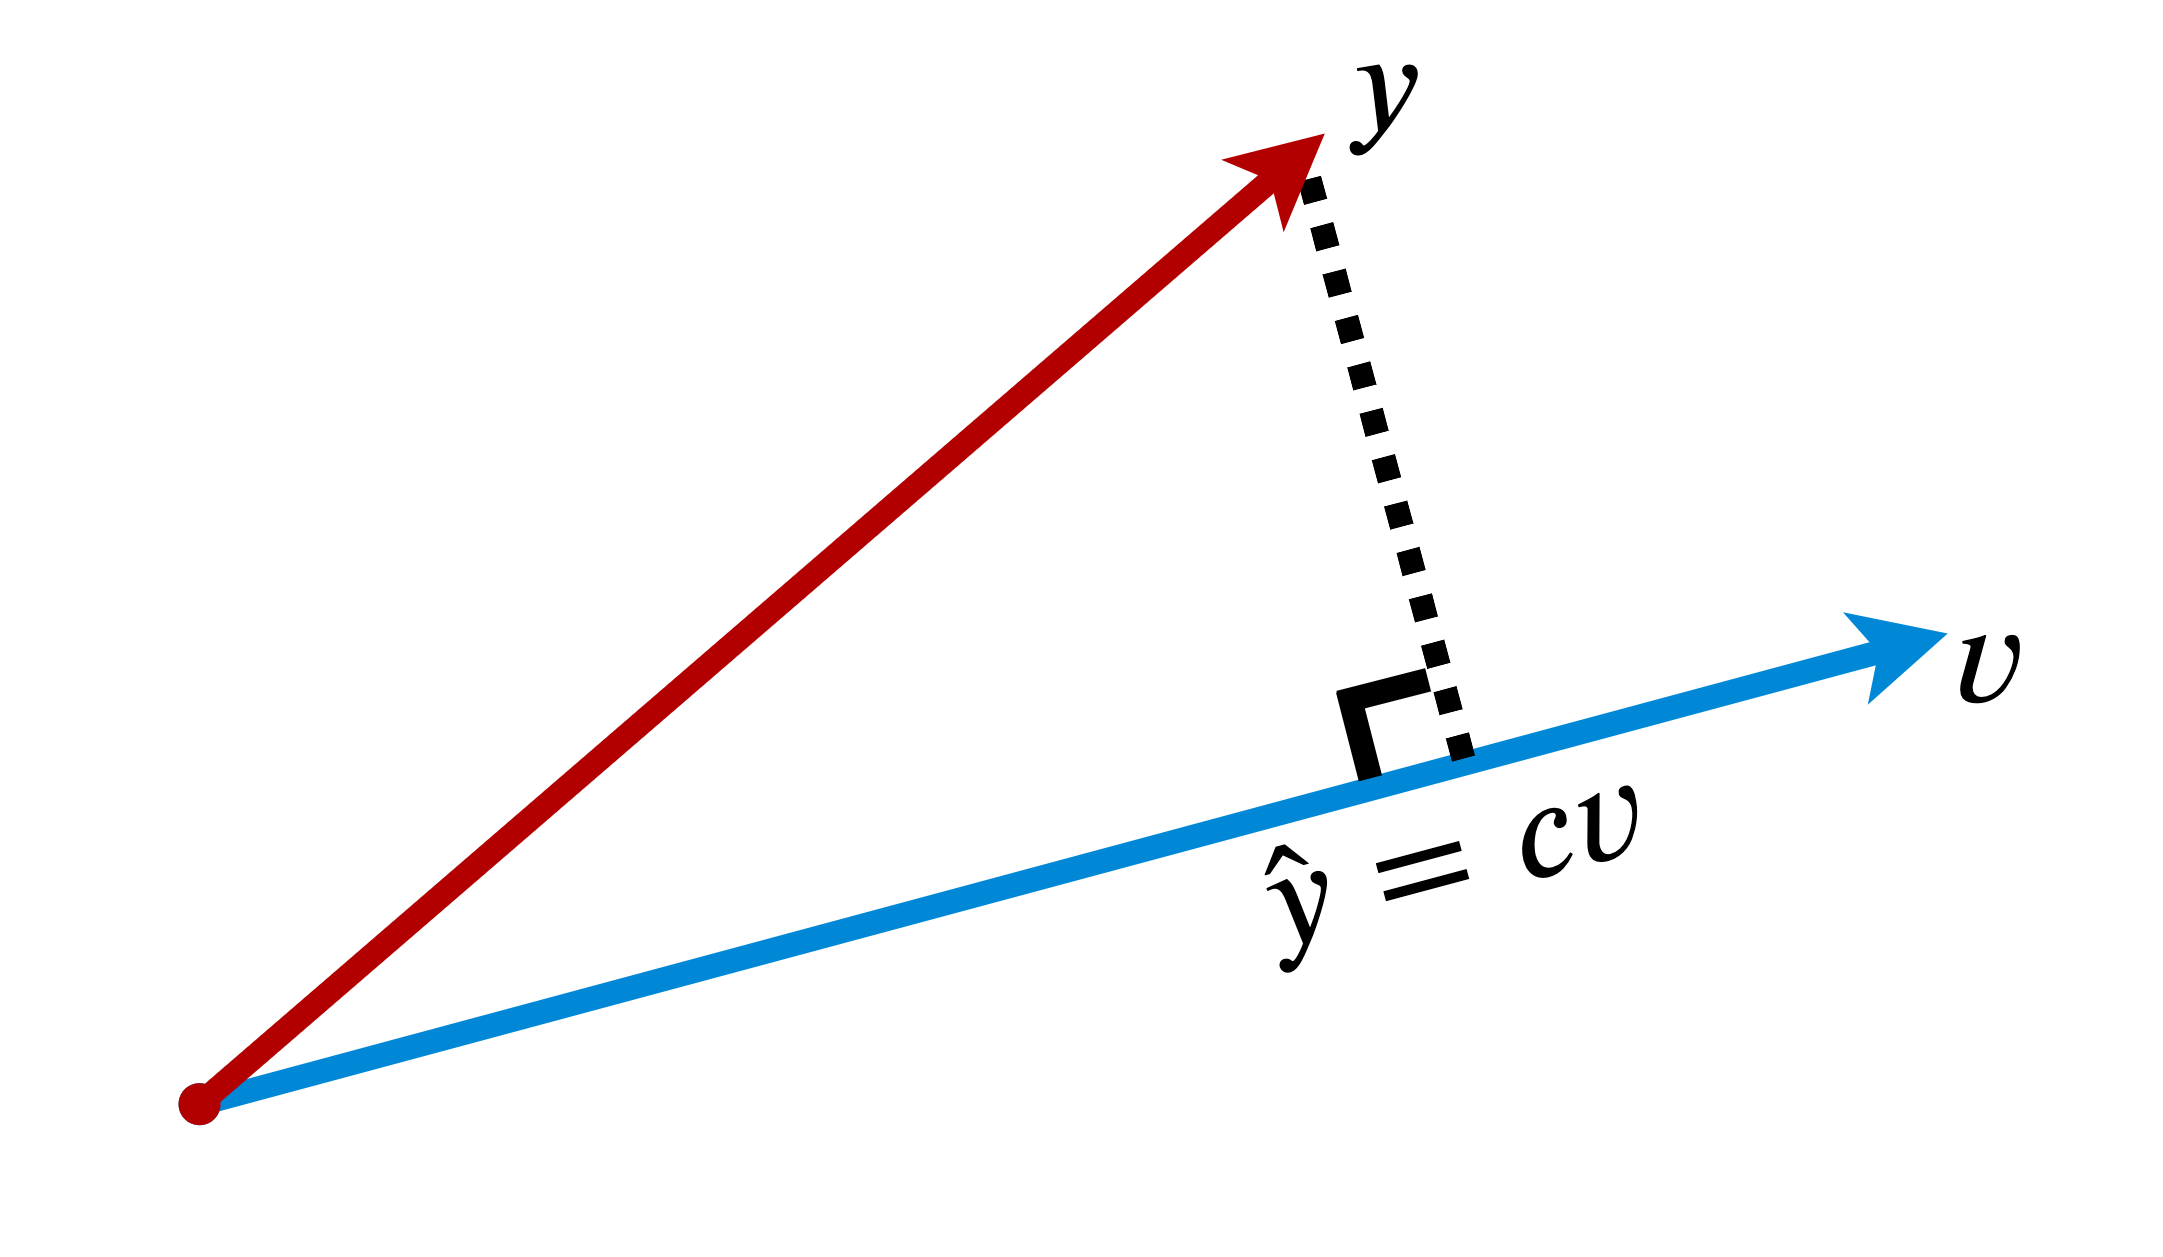
\includegraphics[width=1\linewidth]{images/slider_bg2}

A \href{https://twitter.com/causalinf/status/1259448663270658050}{list of the 10 most important econometric theorems} was circulated on Twitter, based on what Jeffrey Wooldridge claims are the bases for most econometrics. As a political scientist with applied statistics training, this list caught my attention because it contains many of the theorems I see used in (methods) papers, but which I typically glaze over for lack of understanding. The complete list (slightly paraphrased) is:

\begin{enumerate}
\def\labelenumi{\arabic{enumi}.}
\tightlist
\item
  Law of Iterated Expectations, Law of Total Variance
\item
  Linearity of Expectations, Variance of a Sum
\item
  Jensen's Inequality, Chebyshev's Inequality
\item
  Linear Projection and its Properties
\item
  Weak Law of Large Numbers, Central Limit Theorem
\item
  Slutsky's Theorem, Continuous Convergence Theorem, Asymptotic Equivalence Lemma
\item
  Big Op, Little op, and the algebra of them
\item
  Delta Method
\item
  Frisch-Waugh Partialling Out
\item
  For PD matrices A and B, A-B is PSD if and only if \(B^{-1} - A^{-1}\) is PSD.
\end{enumerate}

As an exercise in improving my own knowledge of these fundamentals, I decided to work through each theorem -- using various lecture notes found online, and excellent textbooks like Aronow \& Miller's \citeyearpar{aronow2019foundations} \emph{Foundations of Agnostic Statistics}, Angrist and Pischke's \citeyearpar{angrist2008mostly} \emph{Mostly Harmless Econometrics}, and Wasserman's \citeyearpar{WassermanAllStatisticsConcise2004} \emph{All of Statistics}.

I found for a list of important theorems there were few consistent sources that contained explanations \emph{and} proofs of each item. Often, textbooks had excellent descriptive intuitions but would hold back on offering full, annotated proofs. Or full proofs were offered without explaining the wider significance of the theorems. Some of the concepts, moreover, had different definitions dependent on the field or source of the proof (like Slutsky's Theorems)!

This resource is an attempt to collate my writing on these theorems -- the intuitions, proofs, and examples -- into a single document. I have taken some liberties in doing so -- for instance combining Wooldridge's first two points into a single chapter on `Expectation Theorems', and often omit continuous proofs where discrete proofs are similar and easier to follow. That said, I have tried to be reasonably exhaustive in my proofs so that they are accessible to those (like me) without a formal statistics background.

The inspiration for this project was Jeffrey Wooldridge's list, an academic whose work I admire greatly. This document, however, is in no way endorsed by or associated with him. Most of the applied examples (and invisible corrections to my maths) stem from discussions with Andy Eggers and Musashi Harukawa. There will inevitably still be some errors, omissions, and confusing passages. I would be more than grateful to receive any feedback at \href{mailto:thomas.robinson@durham.ac.uk}{\nolinkurl{thomas.robinson@durham.ac.uk}} or via the \href{github.com/tsrobinson/10EconTheorems}{GitHub repo for this project}.

\hypertarget{prerequisites}{%
\subsection*{Prerequisites}\label{prerequisites}}
\addcontentsline{toc}{subsection}{Prerequisites}

I worked through these proofs learning the bits of maths I needed as I went along. For those who want to consult Google a little less than I had to, the following should ease you into the more formal aspects of this document:

\begin{itemize}
\item
  A simple working knowledge of probability theory
\item
  The basics of expectation notation, but you don't need to know any expectation rules (I cover the important ones in \protect\hyperlink{exp_theorems}{Chapter 1}).
\item
  A basic understanding of linear algebra (i.e.~how you multiply matrices, what transposition is, and what the identity matrix looks like). More complicated aspects like eigenvalues and Gaussian elimination make fleeting appearances, particularly in \protect\hyperlink{pd}{Chapter 9}, but these are not crucial.
\item
  Where relevant, I provide coded examples in R. I've kept my use of packages to a minimum so the code should be reasonably easy to read/port to other programming languages.
\end{itemize}

\hypertarget{version-notes}{%
\subsection*{Version notes}\label{version-notes}}
\addcontentsline{toc}{subsection}{Version notes}

\textbf{v0.1}

This is the first complete draft, and some sections are likely to be changed in future versions. For instance, in \protect\hyperlink{pd}{Chapter 9} I would like to provide a more comprehensive overview of quadratic form in linear algebra, how we derive gradients, and hence the shape of PD matrices. Again, any suggestions on ways to improve/add to this resource are very much welcome!

\href{https://ts-robinson.com/files/_10ET/index.html}{10 Fundamental Theorems for Econometrics} by \href{https://ts-robinson.com}{Thomas Samuel Robinson} is licensed under \href{https://creativecommons.org/licenses/by-nc-sa/4.0/}{CC BY-NC-SA 4.0}


\includegraphics[width=0.89in]{images/cc}

\includegraphics[width=0.89in]{images/by}

\includegraphics[width=0.89in]{images/nc}

\includegraphics[width=0.89in]{images/sa}

\hypertarget{exp_theorems}{%
\chapter{Expectation Theorems}\label{exp_theorems}}

This chapter sets out some of the basic theorems that can be derived from the definition of expectations, as highlighted by Wooldridge. I have combined his first two points into a single overview of expectation maths. The theorems themselves are not as immediately relevant to applied research as some of the later theorems on Wooldridge's list. However, they often form the fundamental basis upon which future proofs are conducted.

\hypertarget{law-of-iterated-expectations}{%
\section{Law of Iterated Expectations}\label{law-of-iterated-expectations}}

The Law of Iterated Expectations (LIE) states that:

\begin{equation}
    \mathbb{E}[X] = \mathbb{E}[\mathbb{E}[X|Y]]
\end{equation}

In plain English, the expected value of \(X\) is equal to the expectation over the conditional expectation of \(X\) given \(Y\). More simply, the mean of X is equal to a weighted mean of conditional means.

Aronow \& Miller \citeyearpar{aronow2019foundations} note that LIE is `one of the most important theorems', because being able to express unconditional expectation functions in terms of conditional expectations allow you to hold some parameters fixed, making calculations more tractable.

\hypertarget{proof-of-lie}{%
\subsection{Proof of LIE}\label{proof-of-lie}}

First, we can express the expectation over conditional expectations as a weighted sum over all possible values of Y, and similarly express the conditional expectations using summation too:

\begin{align}
    \mathbb{E}[\mathbb{E}[X|Y]] &= \sum_y\mathbb{E}[X|Y=y]P(Y=y) \\
          &= \sum_y\sum_x xP(X=x|Y=y)P(Y=y) \label{eq:lie_expand} \\
          &= \sum_y\sum_x xP(Y=y|X=x)P(X=x). \label{eq:lie_bayes},
\end{align}

Note that the final line follows due to Bayes' Rule.\footnote{Bayes' Rule states \(P(A|B) = \frac{P(B|A)P(A)}{P(B)}\). Therefore:
  \begin{equation*}
  P(X=x|Y=y)\times P(Y=y) = \frac{P(Y=y|X=x)P(X=x) P(Y=y)}{P(Y=y)} = P(Y=y|X=x)P(X=x).
  \end{equation*}} And so:

\begin{align}
    ... &= \sum_y\sum_x xP(X=x)P(Y=y|X=x) \label{eq:rearrange}\\
          &= \sum_x xP(X=x) \sum_y P(Y=y|X=x) \label{eq:shift}\\
          &= \sum_x xP(X=x) \label{eq:equals_one}\\
          &= \mathbb{E}[X] \; \; \; \square
\end{align}

The last steps of the proof are reasonably simple. Equation \ref{eq:rearrange} is a trivial rearrangement of terms. The second line follows since \(y\) does not appear in \(xP(X=x)\) and so we can move the summation over \(Y\) to within the summation over \(X\). The final line follows from the fact that the sum of the conditional probabilities \(P(Y=y|X=x)=1\) (by simple probability theory).

\hypertarget{law-of-total-variance}{%
\section{Law of Total Variance}\label{law-of-total-variance}}

The Law of Total Variance (LTV) states the following:
\begin{equation}
    var[Y] = \mathbb{E}[var[Y|X]] + var(\mathbb{E}[Y|X])
\end{equation}

\hypertarget{proof-of-ltv}{%
\subsection{Proof of LTV}\label{proof-of-ltv}}

LTV can be proved almost immediately using LIE and the definition of variance:

\begin{align}
    var(Y) &= \mathbb{E}[Y^2] - \mathbb{E}[Y]^2 \label{eq:var_def} \\ 
           &= \mathbb{E}[\mathbb{E}[Y^2|X]] - \mathbb{E}[\mathbb{E}[Y|X]]^2 \label{eq:var_lie} \\ 
           &= \mathbb{E}[var[Y|X] + \mathbb{E}[Y]^2]] - \mathbb{E}[\mathbb{E}[Y|X]]^2 \label{eq:var_by10}\\
           &= \mathbb{E}[var[Y|X]] + (\mathbb{E}[\mathbb{E}[Y]^2] - \mathbb{E}[\mathbb{E}[Y|X]]^2) \label{eq:var_eshift}\\
           &= \mathbb{E}[var[Y|X]] + var(\mathbb{E}[Y|X]) \label{eq:var_by10_2} \; \; \; \square
\end{align}

The second line applies LIE to both \(Y^2\) and \(Y\) separately. Then we apply the definition of variance to \(\mathbb{E}[Y^2|X]\), and subsequently decompose this term (since \(\mathbb{E}[A+B] = \mathbb{E}[A] + \mathbb{E}[B]\).

\hypertarget{linearity-of-expectations}{%
\section{Linearity of Expectations}\label{linearity-of-expectations}}

The Linearity of Expectations (LOE) simply states that:

\begin{equation}
    \mathbb{E}[aX + bY] = a\mathbb{E}[X] + b\mathbb{E}[Y],
\end{equation}

where \(a\) and \(b\) are real numbers, and \(X\) and \(Y\) are random variables.

\hypertarget{proof-of-loe}{%
\subsection{Proof of LOE}\label{proof-of-loe}}

\begin{align}
    \mathbb{E}[aX + bY] &= \sum_x\sum_y (ax+by) P(X=x, Y=y) \label{eq:loe_sums} \\
    &= \sum_x\sum_y ax P(X=x, Y=y) + \sum_x\sum_y by P(X=x, Y=y) \\
    &= a\sum_x x\sum_y P(X=x, Y=y) + b \sum_y y \sum_x P(X=x, Y=y) \label{eq:loe_rearrange}\\ 
\end{align}

The first line simply expands the expectation into summation form i.e.~the expectation is the sum of \(aX + bY\) for each (discrete) value of \(X\) and \(Y\) weighted by their joint probability. We then expand out these terms. Since summations are commutative, we can rearrange the order of the summations for each of the two parts in the final line, and shift the real numbers and random variables outside the various operators.

Now note that \(\sum_{i} P(I=i, J=j) \equiv P(J=j)\) by probability theory. Therefore:

\begin{align}
    ... &= a\sum_x x P(X=x) + b\sum_y y P(Y = y)
\end{align}

The two terms within summations are just the weighted averages of \(X\) and \(Y\) respectively, i.e.~the expectations of \(X\) and \(Y\), so:

\begin{align}
    ... &= a\mathbb{E}[X] + b\mathbb{E}[Y] \; \; \; \square \\
\end{align}

\hypertarget{variance-of-a-sum}{%
\section{Variance of a Sum}\label{variance-of-a-sum}}

There are two versions of the Variance of a Sum (VOS) law:

\begin{itemize}
\tightlist
\item
  \(var(X + Y) = var(X) + var(Y),\) when X and Y are independent
\item
  \(var(X+Y) = var(X) + var(Y) + 2Cov(X,Y)\), when X and Y are correlated
\end{itemize}

\hypertarget{proof-of-vos-x-y-are-independent}{%
\subsection{\texorpdfstring{Proof of VoS: \(X, Y\) are independent}{Proof of VoS: X, Y are independent}}\label{proof-of-vos-x-y-are-independent}}

\begin{align}
    var(X + Y) &= \mathbb{E}[(X+Y)^2] - (\mathbb{E}[X+Y])^2 \\
    &= \mathbb{E}[(X^2 + 2XY + Y^2)] - (\mathbb{E}[X] + \mathbb{E}[Y])^2
\end{align}

The first line of the proof is simply the definition of variance. In the second line, we expand the equation in the first term and using LOE decompose the second term. We can expand this equation further, continuing to use LOE and noting that :

\begin{align}
    ... &= \mathbb{E}[X^2] + \mathbb{E}[2XY] + \mathbb{E}[Y^2] - (\mathbb{E}[X]^2 + 2\mathbb{E}[X]\mathbb{E}[Y] + \mathbb{E}[Y]^2)\\
     &= \mathbb{E}[X^2] + \mathbb{E}[Y^2] - \mathbb{E}[X]^2 - \mathbb{E}[Y]^2 \\
     &= Var[X] + Var[Y] \; \; \; \square
\end{align}

since \(\mathbb{E}[A]\mathbb{E}[B] = \mathbb{E}[AB]\) when \(A\) and \(B\) are independent.

\hypertarget{proof-of-vos-x-y-are-dependent}{%
\subsection{\texorpdfstring{Proof of VoS: \(X, Y\) are dependent}{Proof of VoS: X, Y are dependent}}\label{proof-of-vos-x-y-are-dependent}}

As before, we can expand out the variance of a sum into its expected values:

\begin{align}
    var(X + Y) &= \mathbb{E}[X^2] + \mathbb{E}[2XY] + \mathbb{E}[Y^2] - (\mathbb{E}[X]^2 + 2\mathbb{E}[X]\mathbb{E}[Y] + \mathbb{E}[Y]^2).
\end{align}

Since \(X\) and \(Y\) are assumed to be dependent, the non-squared terms do not necessarily cancel each other out anymore. Instead, we can rearrange as follows:

\begin{align}
    var(X + Y) &= var(X) + var(Y) + \mathbb{E}[2XY] - 2\mathbb{E}[X]\mathbb{E}[Y]\\
    & = var(X) + var(Y) + 2(\mathbb{E}[XY] - \mathbb{E}[X]\mathbb{E}[Y]),
\end{align}

and note that \(\mathbb{E}[AB]-\mathbb{E}[A]\mathbb{E}[B] = Cov(A,B)\):

\begin{equation}
... = var(X) + var(Y) + 2Cov(A,B) \; \; \; \square
\end{equation}

Two further points are worth noting. First, the independent version of the proof is just a special case of the dependent version of the proof. When \(X\) and \(Y\) are independent, the covariance between the two random variables is zero, and therefore the the variance of the sum is just equal to the sum of the variances.

Second, nothing in the above proofs rely on there being just two random variables. In fact, \(var(\sum^n_i X_i) = \sum^n_ivar(X_i)\) when all variables are independent from each other, and equal to \(\sum^n_ivar(X_i) + 2\sum^n_{1 \leq i < j \leq n}Cov(X_i,X_j).\) This can be proved by induction using the above proofs, but intuitively: we can replace, for example, \(Y\) with \(Y = (Y_1 + Y_2)\) and iteratively apply the above proof first to \(X+Y\) and then subsequently expand \(var(Y)\) as \(var(Y_1+Y_2)\).

\hypertarget{exp_ineq}{%
\chapter{Inequalities involving expectations}\label{exp_ineq}}

This chapter discusses and proves two inequalities that Wooldridge highlights - Jensen's and Chebyshev's. Both involve expectations (and the theorems derived in the previous chapter).

\hypertarget{jensens-inequality}{%
\section{Jensen's Inequality}\label{jensens-inequality}}

Jensen's Inequality is a statement about the relative size of the expectation of a function compared with the function over that expectation (with respect to some random variable). To understand the mechanics, I first define convex functions and then walkthrough the logic behind the inequality itself.

\hypertarget{convex-functions}{%
\subsection{Convex functions}\label{convex-functions}}

A function \(f\) is convex (in two dimensions) if all points on a straight line connecting any two points on the graph of \(f\) is above or on that graph. More formally, \(f\) is convex if for \(\forall x_1, x_2 \in \mathbb{R}\), and \(\forall t \in [0,1]\):

\[
    f(tx_1, (1-t)x_2) \leq tf(x_1) + (1-t)f(x_2).
\]

Here, \(t\) is a weighting parameter that allows us to range over the full interval between points \(x_1\) and \(x_2\).

Note also that concave functions are defined as the opposite of convex functions i.e.~a function \(h\) is concave if and only if \(-h\) is convex.

\hypertarget{the-inequality}{%
\subsection{The Inequality}\label{the-inequality}}

Jensen's Inequality (JI) states that, for a convex function \(g\) and random variable \(X\):

\[
    \mathbb{E}[g(X)] \geq g(E[X])
\]

This inequality is exceptionally general -- it holds for any convex function. Moreover, given that concave functions are defined as negative convex functions, it is easy to see that JI also implies that if \(h\) is a \textit{concave} function, \(h(\mathbb{E}[X]) \geq \mathbb{E}[h(X)]\).\footnote{Since \(-h(x)\) is convex, \(\mathbb{E}[-h(X)] \geq -h(\mathbb{E}[X])\) by JI. Hence, \(h(\mathbb{E}[X]) - \mathbb{E}[h(X)] \geq 0\) and so \(h(\mathbb{E}[X]) \geq \mathbb{E}[h(X)]\).}

Interestingly, note the similarity between this inequality and the definition of variance in terms of expectations:

\[
    var(X) = \mathbb{E}[X^2] - (\mathbb{E}[X])^2,
\]

and since \(var(X)\) is always positive:

\[
\begin{aligned}
    \mathbb{E}[X^2] -  (\mathbb{E}[X])^2 &\geq 0 \\
    \mathbb{E}[X^2] &\geq (\mathbb{E}[X])^2).
\end{aligned}
\]

We can therefore define \(g(X) = X^2\) (a convex function), and see that variance itself is an instance of Jensen's Inequality.

\hypertarget{proof_ji}{%
\subsection{Proof}\label{proof_ji}}

Assume \(g(X)\) is a convex function, and \(L(X)= a + bX\) is a linear function tangential to \(g(X)\) at point \(\mathbb{E}[X]\).

Hence, since \(g\) is convex and \(L\) is tangential to \(g\), we know by definition that:

\begin{equation}
    g(x) \geq L(x), \forall x \in X.
\end{equation}

So, therefore:

\begin{align}
    \mathbb{E}[g(X)] &\geq \mathbb{E}[L(X)] \\
    &\geq \mathbb{E}[A + bX] \label{eq:def_of_L} \\
    &\geq a +b\mathbb{E}[X] \label{eq:loe}\\ 
    &\geq L(\mathbb{E}[X]) \label{eq:def_of_L2}\\
    &\geq g(\mathbb{E}[X]) \; \; \; \square \label{eq:tang}
\end{align}

The majority of this proof is straightforward. If one function is always greater than or equal to another function, then the unconditional expectation of the first function must be at least as big as that of the second. The interior lines of the proof follow from the definition of \(L\), the linearity of expectations, and another application of the definition of \(L\) respectively.

The final line then follows because, by the definition of the straight line \(L\), we know that \(L[\mathbb{E}[X]]\) is tangential with \(g\) at \(\mathbb{E}[\mathbb{E}[X]] = \mathbb{E}[X] = g(\mathbb{E}[X])\).\footnote{Based on \href{http://www.stat.cmu.edu/~larry/=stat705/Lecture2.pdf}{lecture notes} by Larry Wasserman.}

\hypertarget{application}{%
\subsection{Application}\label{application}}

In Chapter 2 of \emph{Agnostic Statistics} \citeyearpar{aronow2019foundations}, the authors note (almost in passing) that the standard error of the mean is not unbiased, i.e.~that \(\mathbb{E}[\hat{\sigma}] \neq \sigma\), even though it is consistent i.e.~that \(\hat{\sigma}\xrightarrow{p} \sigma.\) The bias of the mean's standard error is somewhat interesting (if not surprising), given how frequently we deploy the standard error (and, in a more general sense, highlights how important asymptotics are not just for the estimation of parameters, but also those parameters' uncertainty). The proof of why \(\hat{\sigma}\) is biased also, conveniently for this chapter, uses Jensen's Inequality.

The standard error of the mean is denoted as

\[\sigma =  \sqrt{V(\bar{X})}\],

where \(V(\bar{X}) = \frac{V(X)}{n}\).

Our best estimate of this quantity \(\hat{\sigma} = \sqrt{\hat{V}(\bar{X})}\) is simply the square root of the sample variance estimator. We know that the variance estimator itself is unbiased and a consistent estimator of the sampling variance (see \emph{Agnostic Statistics} Theorem 2.1.9).

The bias in the estimate of the sample mean's standard error originates from the square root function Note that the square root is a strictly concave function. This means we can make two claims about the estimator. First, as with any concave function we can use the inverse version of Jensen's Inequality, i.e.~that \(\mathbb{E}[g(X)] \leq g(\mathbb{E}[X])\). Second, since the square root is a \emph{strictly} concave function, we can use the weaker ``less than or equal to'' operator with the strict ``less than'' inequality. Hence, the proof is reasonably easy:

\[
\begin{aligned}
\mathbb{E}\left[\hat{\sigma}\right] = \mathbb{E}\left[\sqrt{\hat{V}(\bar{X})}\right] &< \sqrt{\mathbb{E}[\hat{V}(\bar{X})]} \;\;\; \text{(by Jensen's Inequality)}\\
& < \sqrt{V(\bar{X})} \;\;\; \text{(since the sampling variance is unbiased)} \\
& < \sigma. \;\;\; \square
\end{aligned}
\]

The first line follows by first defining the conditional expectation of the sample mean's standard error, and then applying the noted variant of Jensen's inequality. Then, since we know that the standard error estimator of the variance is unbiased, we can replace the expectation with the true sampling variance, and note finally that the square root of the true sampling variance is, by definition, the true standard error of the sample mean. Hence, we see that our estimator of the sampling mean's standard error is strictly less than the true value and therefore is biased.

\hypertarget{chebyshevs-inequality}{%
\section{Chebyshev's Inequality}\label{chebyshevs-inequality}}

The other inequality Wooldridge highlights is the Chebyshev Inequality. This inequality states that for a set of probability distributions, no more than a specific proportion of that distribution is more than a set distance from the mean.

More formally, if \(\mu = \mathbb{E}[X]\) and \(\sigma^2 = var(X)\), then:

\begin{equation}
    %P(|X-\mu|\geq t) \leq \frac{\sigma^2}{t^2} \text{ and }
    P(|Z| \geq k) \leq \frac{1}{k^2}, 
\end{equation}

where \(Z = (X-\mu)/\sigma\) \citep[p.64]{WassermanAllStatisticsConcise2004} and \(k\) indicates the number of standard deviations.

\hypertarget{proof}{%
\subsection{Proof}\label{proof}}

First, let us define the variance (\(\sigma^2\)) as:

\begin{equation}
    \sigma^2 = \mathbb{E}[(X-\mu)^2].
\end{equation}

By expectation theory, we know that we can express any unconditional expectation as the weighted sum of its conditional components i.e.~\(\mathbb{E}[A] = \sum_i\mathbb{E}[A|c_i]P(c_i),\) where \(\sum_iP(c_i)=1\). Hence:

\begin{equation}
    ... = \mathbb{E}[(X-\mu)^2 | k\sigma \leq |X - \mu|]P(k\sigma \leq |X - \mu|) + \mathbb{E}[(X-\mu)^2 | k\sigma > |X - \mu|]P(k\sigma > |X - \mu|) 
\end{equation}

Since any probability is bounded between 0 and 1, and variance must be greater than or equal to zero, the second term must be non-negative. If we remove this term, therefore, the right-hand side is necessarily either the same size or smaller. Therefore we can alter the equality to the following inequality:

\begin{equation}
    \sigma^2 \geq \mathbb{E}[(X-\mu)^2 | k\sigma \leq X - \mu]P(k\sigma \leq |X - \mu|)
\end{equation}

This then simplifies:

\[
\begin{aligned}
    \sigma^2 &\geq (k\sigma)^2P(k\sigma \leq |X - \mu|) \\
    &\geq k^2\sigma^2P(k\sigma \leq |X - \mu|) \\
    \frac{1}{k^2} &\geq P(|Z| \geq k) \; \; \; \square
\end{aligned}
\]

Conditional on \(k\sigma \leq |X-\mu|\), \((k\sigma)^2 \leq (X-\mu)^2\), and therefore \(\mathbb{E}[(k\sigma)^2] \leq \mathbb{E}[(X-\mu)^2]\). Then, the last step simply rearranges the terms within the probability function.\footnote{\(k\sigma \leq |X-\mu| \equiv k \leq |X-\mu|/\sigma \equiv |Z| \geq k,\) since \(\sigma\) is strictly non-negative.}

\hypertarget{applications}{%
\subsection{Applications}\label{applications}}

Wasserman notes that this inequality is useful when we want to know the probable bounds of an unknown quantity, and where direct computation would be difficult. It can also be used to prove the Weak Law of Large Numbers (point 5 in Wooldridge's list!) I delay discussion of this application until Section X.

It is worth noting, however, that the inequality is really powerful -- it guarantees that a certain amount of a probability distribution is within a certain region -- irrespective of the shape of that distribution (so long as we can estimate the mean and variance)!

For some well-defined distributions, this theorem is weaker than what we know by dint of their form. For example, we know that for a normal distribution, approximately 95 percent of values lie within 2 standard deviations of the mean. Chebyshev's Inequality only guarantees that 75 percent of values lie within two standard deviations of the mean (since \(P(|Z| \geq k) \leq \frac{1}{2^2}\)). Crucially, however, even if we didn't know whether a given distribution was normal, so long as it is a well-behaved probability distribution (i.e.~the unrestricted integral sums to 1) we can guarantee that 75 percent will lie within two standard deviations of the mean.

\hypertarget{linear_projection}{%
\chapter{Linear Projection}\label{linear_projection}}

This chapter provides a basic introduction to projection using both linear algebra and geometric demonstrations. I discuss the derivation of the orthogonal projection, its general properties as an ``operator'', and explore its relationship with ordinary least squares (OLS) regression. I defer a discussion of linear projections' applications until the \protect\hyperlink{frisch}{penultimate chapter} on the Frisch-Waugh Theorem, where projection matrices feature heavily in the proof.

\hypertarget{proj_def}{%
\section{Projection}\label{proj_def}}

Formally, a projection \(P\) is a linear function on a vector space, such that when it is applied to itself you get the same result i.e.~\(P^2 = P\).\footnote{Since \(P\) is (in the finite case) a square matrix, a projection matrix is an idempotent matrix -- I discuss this property in more detail later on in this note.}

This definition is slightly intractable, but the intuition is reasonably simple. Consider a vector \(v\) in two-dimensions. \(v\) is a finite straight line pointing in a given direction. Suppose there is some point \(x\) not on this straight line but in the same two-dimensional space. The projection of \(x\), i.e.~\(Px\), is a function that returns the point ``closest'' to \(x\) along the vector line \(v\). Call this point \(\bar{x}\). In most contexts, closest refers to Euclidean distance, i.e.~\(\sqrt{\sum_{i} (x_i - \bar{x}_i)^2},\) where \(i\) ranges over the dimensions of the vector space (in this case two dimensions).{[}fn\^{}euclid{]} Figure @ref(fig:lp\_basic) depicts this logic visually. The green dashed line shows the orthogonal projection, and red dashed lines indicate other potential (non-orthgonal) projections that are further away in Euclidean space from \(x\) than \(\bar{x}\).

\begin{figure}
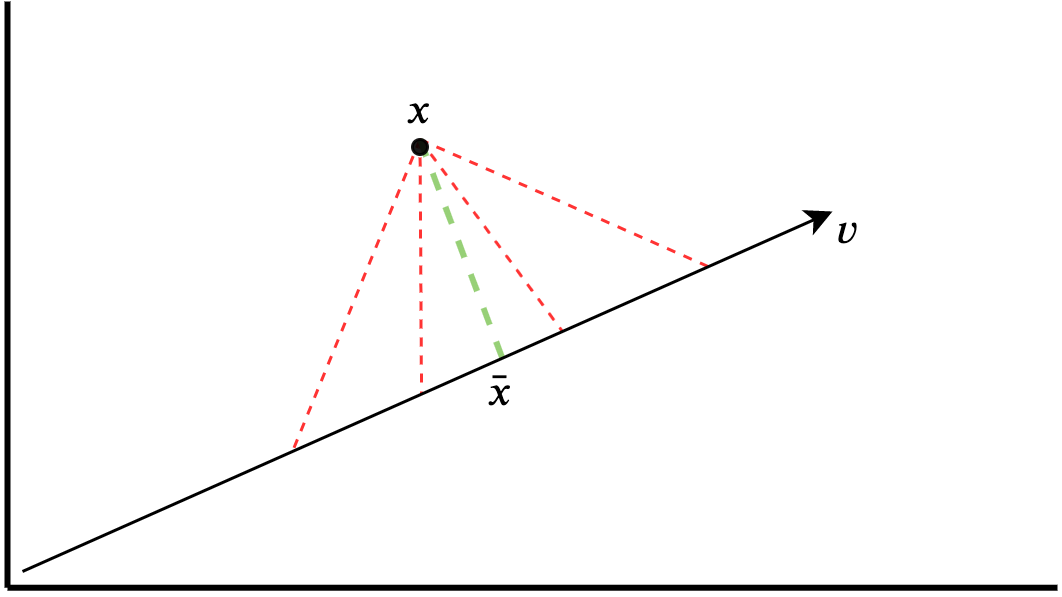
\includegraphics[width=1\linewidth]{images/lp_basic} \caption{Orthogonal projection of a point onto a vector line.}\label{fig:lp-basic}
\end{figure}

In short, projection is a way of simplifying some n-dimensional space -- compressing information onto a (hyper-) plane. This is useful especially in social science settings where the complexity of the phenomena we study mean exact prediction is impossible. Instead, we often want to construct models that compress busy and variable data into simpler, parsimonious explanations. Projection is the statistical method of achieving this -- it takes the full space and simplifies it with respect to a certain number of dimensions.

While the above is (reasonably) intuitive it is worth spelling out the maths behind projection, not least because it helps demonstrate the connection between linear projection and linear regression.

To begin, we can take some point in n-dimensional space, \(x\), and the vector line \(v\) along which we want to project \(x\). The goal is the following:

\[
\begin{aligned}
{arg\,min}_c \sqrt{\sum_{i} (\bar{x}_i - x)^2} & = {arg\,min}_c \sum_{i} (\bar{x}_i - x)^2 \\
& = {arg\,min}_c \sum_{i} (cv_i - x)^2
\end{aligned}
\]

This rearrangement follows since the square root is a monotonic transformation, such that the optimal choice of \(c\) is the same across both \(arg\;min\)'s. Since any potential \(\bar{x}\) along the line drawn by \(v\) is some scalar multiplication of that line (\(cv\)), we can express the function to be minimised with respect to \(c\), and then differentiate:

\[
\begin{aligned}
\frac{d}{dc} \sum_{i} (cv_i - x)^2 & = \sum_{i}2v_i(cv_i - x) \\
& = 2(\sum_{i}cv_i^2  - \sum_{i}v_ix) \\
& = 2(cv'v - v'x) \Rightarrow 0
\end{aligned}
\]

Here we differentiate the equation and rearrange terms. The final step simply converts the summation notation into matrix multiplication. Solving:

\[
\begin{aligned}
2(cv'v - v'x) &= 0 \label{eq:dc_equal_zero} \\ 
cv'v - v'x &= 0 \\
cv'v &= v'x \\
c &= (v'v)^{-1}v'x.
\end{aligned}
\]

From here, note that \(\bar{x}\), the projection of \(x\) onto the vector line, is \(vc = v(v'v)^{-1}v'x.\) Hence, we can define the projection matrix of \(x\) onto \(v\) as:

\[ P_v = v(v'v)^{-1}v'.\]

In plain English, for any point in some space, the orthogonal projection of that point onto some subspace, is the point on a vector line that minimises the Euclidian distance between itself and the original point. A visual demonstration of this point is shown and discussed in Figure \ref{fig:lp-demo} below.

Note also that this projection matrix has a clear analogue to the linear algebraic expression of linear regression. The vector of coefficients in a linear regression \(\hat{\beta}\) can be expressed as \((X′X)^{-1}X′y\). And we know that multiplying this vector by the matrix of predictors \(X\) results in the vector of predicted values \(\hat{y}\). Now we have \(\hat{y} = X(X'X)^{-1}X'Y \equiv P_Xy\). Clearly, therefore, linear projection and linear regression are closely related -- and I return to this point \protect\hyperlink{lp_lr}{below}.

\hypertarget{proj_prop}{%
\section{Properties of the projection matrix}\label{proj_prop}}

The projection matrix \(P\) has several interesting properties. First, and most simply, the projection matrix is square. Since \(v\) is of some arbitrary dimensions \(n \times k\), its transpose is of dimensions \(k \times n\). By linear algebra, the shape of the full matrix is therefore \(n \times n\), i.e.~square.

Projection matrices are also symmetric, i.e.~\(P = P'\). To prove symmetry, note that transposing both sides of the projection matrix definition:

\begin{align}
P' &= (v(v'v)^{-1}v')' \\
&= v(v'v)^{-1}v'\\
&= P,
\end{align}

since \((AB)'=B'A'\) and \((A^{-1})' = (A')^{-1}.\)

Projection matrices are idempotent:

\begin{align}
PP &= v(v'v)^{-1}v'v(v'v)^{-1}v' \\
&= v(v'v)^{-1}v'\\
&= P,
\end{align}

since \((A)^{-1}A = I\) and \(BI = B\).

Since, projection matrices are idempotent, this entails that projecting a point already on the vector line will just return that same point. This is fairly intuitive: the closest point on the vector line to a point already on the vector line is just that same point.

Finally, we can see that the projection of any point is orthogonal to the respected projected point on vector line. Two vectors are orthogonal if \(ab = 0\). Starting with the expression in Equation \ref{eq:dc_equal_zero} (i.e.~minimising the Euclidean distance with respect to \(c\)):

\[
\begin{aligned}
2(cv'v - v'x) &= 0 \\ 
v'cv - v'x &= 0 \\
v'(cv-x) &= 0 \\
v'(\bar{x} - x) &= 0,
\end{aligned}
\]

hence the line connecting the original point \(x\) is orthogonal to the vector line.

The projection matrix is very useful in other fundamental theorems in econometrics, like Frisch Waugh Lovell Theorem discussed in \protect\hyperlink{frisch}{Chapter 8}.

\hypertarget{lp_lr}{%
\section{Linear regression}\label{lp_lr}}

Given a vector of interest, how do we capture as much information from it as possible using set of predictors? Projection matrices essentially simplify the dimensionality of some space, by casting points onto a lower-dimensional plane. Think of it like capturing the shadow of an object on the ground. There is far more detail in the actual object itself but we roughly know its position, shape, and scale from the shadow that's cast on the 2d plane of the ground.

Note also this is actually quite similar to how we think about regression. Loosely, when we regress \(Y\) on \(X\), we are trying to characterise how the components (or predictors) within \(X\) characterise or relate to \(Y\). Of course, regression is also imperfect (after all, the optimisation goal is to minimise the errors of our predictions). So, regression also seems to capture some lower dimensional approximation of an outcome.

In fact, linear projection and linear regression are very closely related. In this final section, I outline how these two statistical concepts relate to each other, both algebraically and geometrically,

Suppose we have a vector of outcomes \(y\), and some n-dimensional matrix \(X\) of predictors. We write the linear regression model as:

\begin{equation}
y = X\beta + \epsilon,
\end{equation}

where \(\beta\) is a vector of coefficients, and \(\epsilon\) is the difference between the prediction and the observed value in \(y\). The goal of linear regression is to minimise the sum of the squared residuals:

\[
arg\,min \,\,  \epsilon^2 = arg\,min (y - X\beta)'(y-X\beta)
\]

Differentiating with respect to \beta and solving:
\[
\begin{aligned}
\frac{d}{d\beta} (y - X\beta)'(y-X\beta) &= -2X(y - X\beta) \\
&= 2X'X\beta -2X'y \Rightarrow 0 \\
X'X\hat{\beta} &= X'y \\
(X'X)^{-1}X'X\hat{\beta} &= (X'X)^{-1}X'y \\
\hat{\beta} &= (X'X)^{-1}X'y.
\end{aligned}
\]

To get our prediction of \(y\), i.e.~\(\hat{y}\), we simply multiply our beta coefficient by the matrix X:

\[
  \hat{y} = X(X'X)^{-1}X'y.
\]

Note how the OLS derivation of \(\hat{y}\) is very similar to \(P = X(X'X)^{-1}X\), the orthogonal prediction matrix. The two differ only in that that \(\hat{y}\) includes the original outcome vector \(y\) in its expression. But, note that \(Py = X(X'X)^{-1}X'y = \hat{y}\)! Hence the predicted values from a linear regression simply are an orthogonal projection of \(y\) onto the space defined by \(X\).

\hypertarget{geometric-interpretation}{%
\subsection{Geometric interpretation}\label{geometric-interpretation}}

It should be clear now that linear projection and linear regression are connected -- but it is probably less clear \emph{why} this holds. To understand what's going on, let's depict the problem geometrically.\footnote{This final section borrows heavily from \href{https://www.youtube.com/watch?v=My51wdv2Uz0}{Ben Lambert's explanation of projection} and a \href{http://andy.egge.rs/teaching/ols_projection.html}{demonstration using R by Andy Eggers}.}

To appreciate what's going on, we first need to invert how we typically think about observations, variables and datapoints. Consider a bivariate regression problem with three observations. Our data will include three variables: a constant (c, a vector of 1's), a predictor (X), and an outcome variable (Y). As a matrix, this might look something like the following:

\begin{longtable}[]{@{}ccc@{}}
\toprule
Y & X & c\tabularnewline
\midrule
\endhead
2 & 3 & 1\tabularnewline
3 & 1 & 1\tabularnewline
2 & 1 & 1\tabularnewline
\bottomrule
\end{longtable}

Typically we would represent the relationship geometrically by treating the variables as dimensions, such that every datapoint is an observation (and we would typically ignore the constant column since all its values are the same).

An alternative way to represent this data is to treat each observation (i.e.~row) as a dimension and then represent each variable as a vector. What does that actually mean? Well consider the column \(Y = (2,3,2)\). This vector essentially gives us the coordinates for a point in three-dimensional space: \(d_1 = 2, d_2 = 3, d_3 = 2\). Drawing a straight line from the origin (0,0,0) to this point gives us a vector line for the outcome. While visually this might seem strange, from the perspective of our data it's not unusual to refer to each variable as a column vector, and that's precisely because it is a quantity with a magnitude and direction (as determined by its position in \(n\) dimensions).

Our predictors are the vectors \(X\) and \(c\) (note the vector \(c\) is now slightly more interesting because it is a diagonal line through the three-dimensional space). We can extend either vector line by multiplying it by a constant e.g.~\(2X = (6,2,2)\). With a single vector, we can only move forwards or backwards along a line. But if we combine two vectors together, we can actually reach lots of points in space. Imagine placing the vector \(X\) at the end of the \(c\). The total path now reaches a new point that is not intersected by either \(X\) or \(c\). In fact, if we multiply \(X\) and \(c\) by some scalars (numbers), we can snake our way across a whole array of different points in three-dimensional space. Figure \ref{fig:lp-span} demonstrates some of these combinations in the two dimensional space created by \(X\) and \(c\).

\begin{figure}
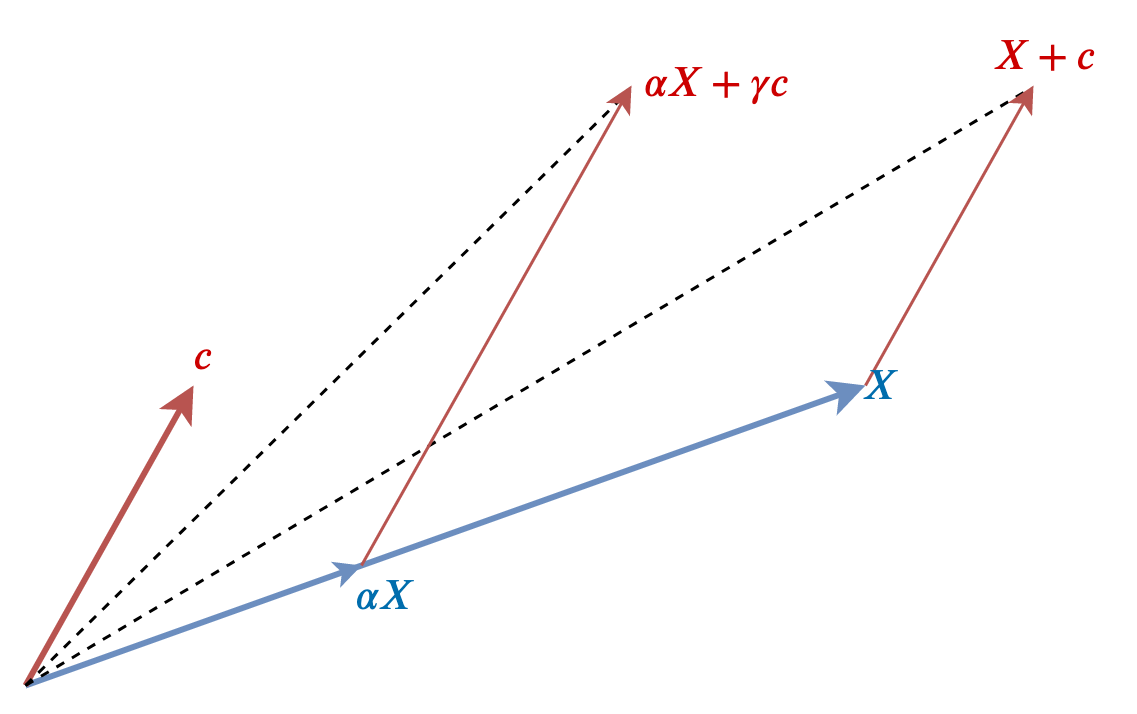
\includegraphics[width=1\linewidth]{images/span} \caption{Potential combinations of two vectors.}\label{fig:lp-span}
\end{figure}

The comprehensive set of all possible points covered by linear combinations of \(X\) and \(c\) is called the \emph{span} or \emph{column space}. In fact, with the specific set up of this example (3 observations, two predictors), the span of our predictors is a flat plane. Imagine taking a flat bit of paper and aligning one corner with the origin, and then angling surface so that the end points of the vectors \(X\) and \(c\) are both resting on the card's surface. Keeping that alignment, any point on the surface of the card is reachable by some combination of \(X\) and \(c\). Algebraically we can refer to this surface as \(col(X,c)\), and it generalises beyond two predictors (although this is much harder to visualise).

Crucially, in our reduced example of three-dimensional space, there are points in space not reachable by combining these two vectors (any point above or below the piece of card). We know, for instance that the vector line \(y\) lies off this plane. The goal therefore is to find a vector that is on the column space of \((X,c)\) that gets closest to our off-plane vector \(y\) as possible. Figure \ref{fig:lp-demo1} depicts this set up visually -- each dimension is an observation, each column in the matrix is represented a vector, and the column space of \((X,c)\) is the shaded grey plane. The vector \(y\) lies off this plane.

\begin{figure}
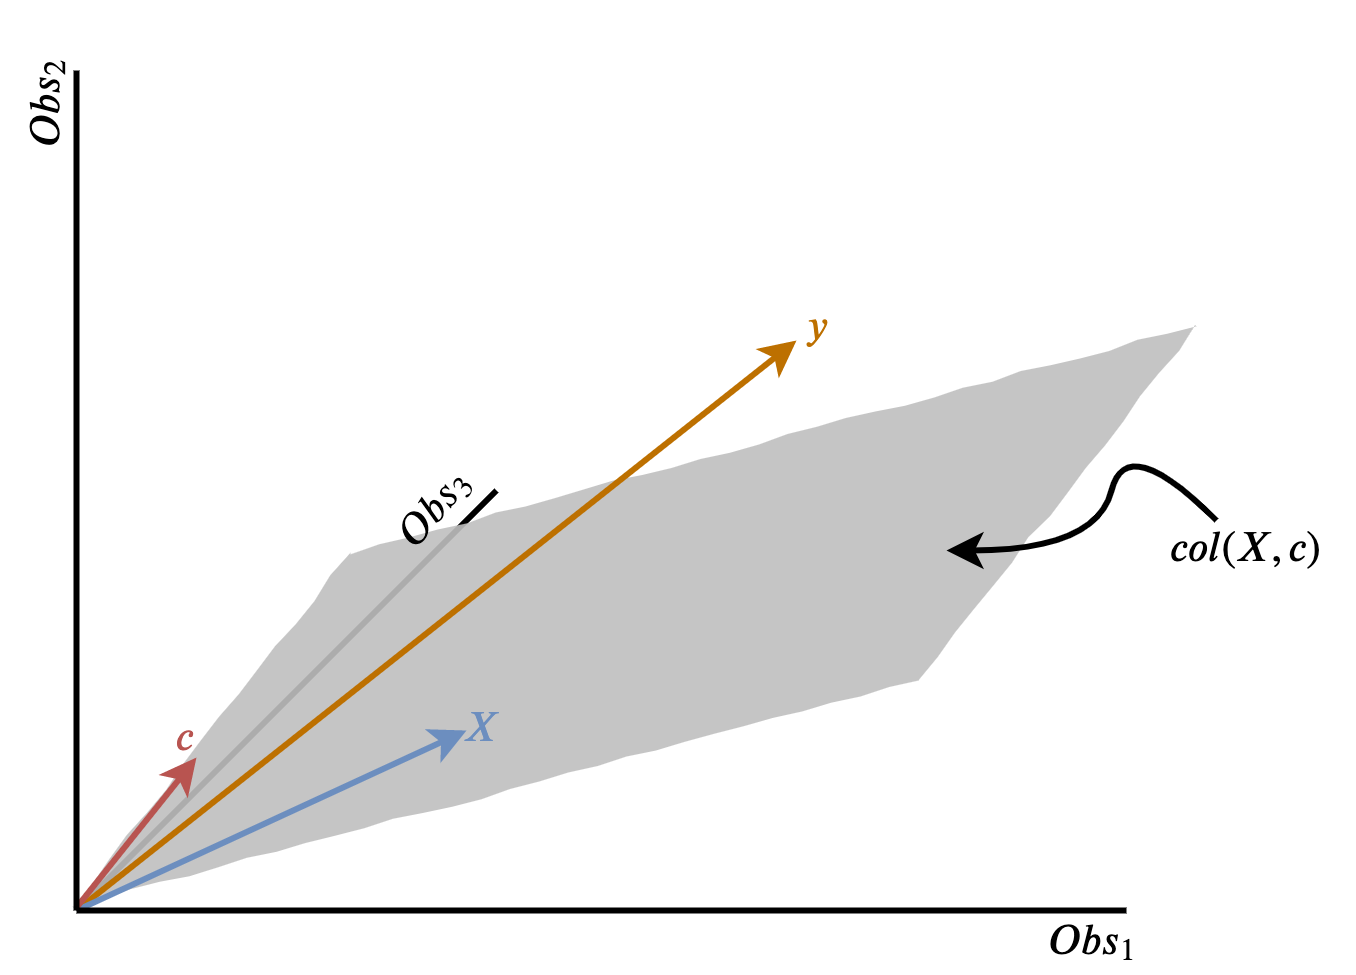
\includegraphics[width=1\linewidth]{images/lp_solve1} \caption{Schematic of orthogonal projection as a geometric problem}\label{fig:lp-demo1}
\end{figure}

From our discussion in \protect\hyperlink{proj_def}{Section 3.1}, we know that the ``best'' vector is the orthogonal projection from the column space to the vector \(y\). This is the shortest possible distance between the flat plane and the observed outcome, and is just \(\hat{y}\). Moreover, since \(\hat{y}\) lies on the column space, we know we only need to combine some scaled amount of \(X\) and \(c\) to define the vector \(\hat{y}\), i.e., \(\beta_1X + \beta_0c\). Figure \ref{fig:lp-demo2} shows this geometrically. And in fact, the scalar coefficients \(\beta_1, \beta_0\) in this case are just the regression coefficients derived from OLS. Why? Because we know that the orthogonal projection of \(y\) onto the column space minimises the error between our prediction \(\hat{y}\) and the observed outcome vector \(y\). This is the same as the minimisation problem that OLS solves, as outlined at the beginning of this section!

\begin{figure}
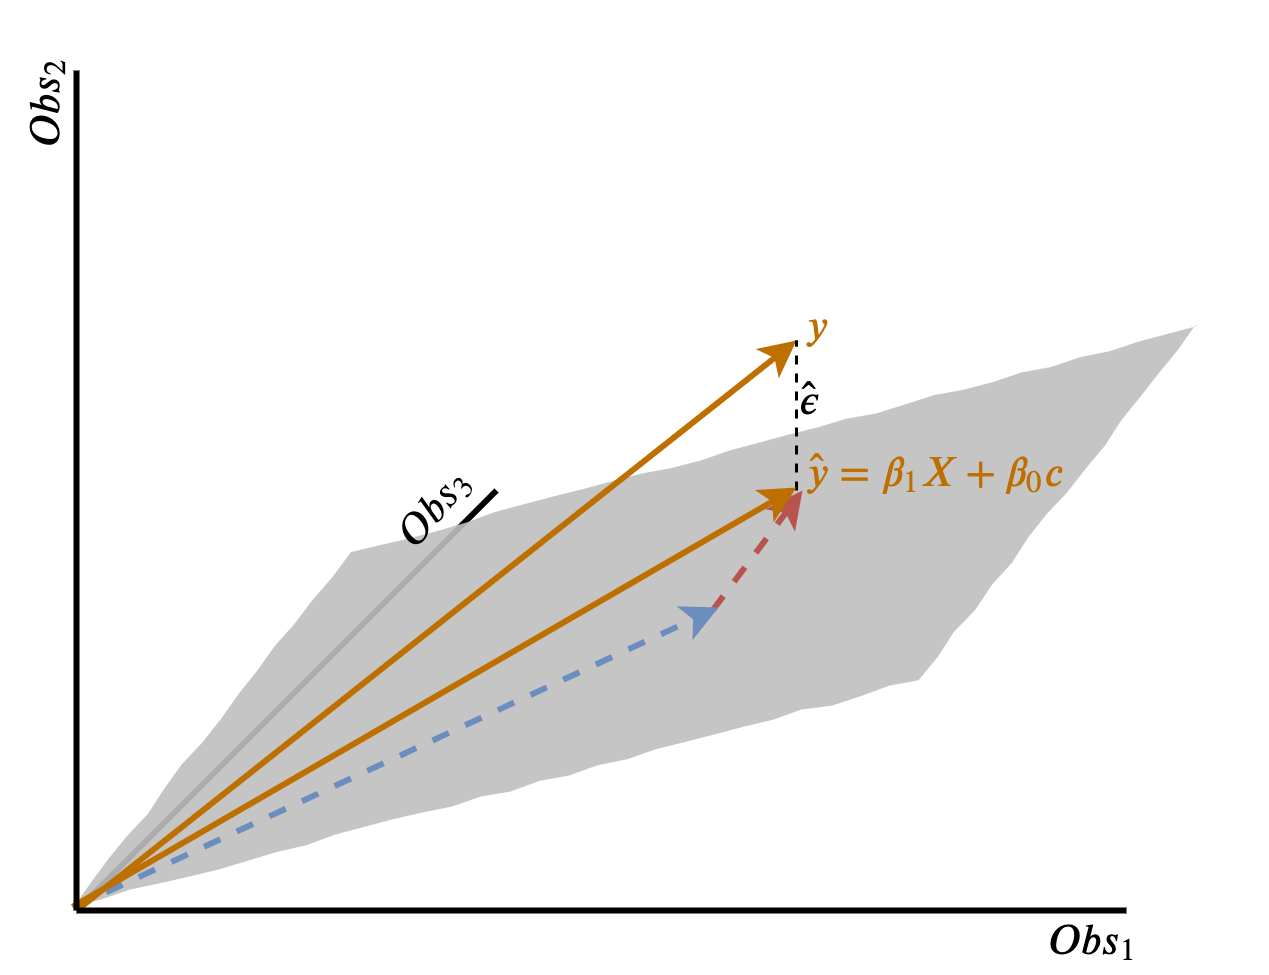
\includegraphics[width=1\linewidth]{images/lp_solve2} \caption{Relation of orthogonal projection to linear regression.}\label{fig:lp-demo2}
\end{figure}

Consider any other vector on the column space, and the distance between itself and and \(y\). Each non-orthogonal vector would be longer, and hence have a larger predictive error, than \(\hat{y}\). For example, Figure \ref{fig:lp-distances} plots two alternative vectors on \(col(X,c)\) alongside \(\hat{y}\). Clearly, \(\hat{\epsilon} < \epsilon' < \epsilon'',\) and this is true of any other vector on the column space too.

\begin{figure}
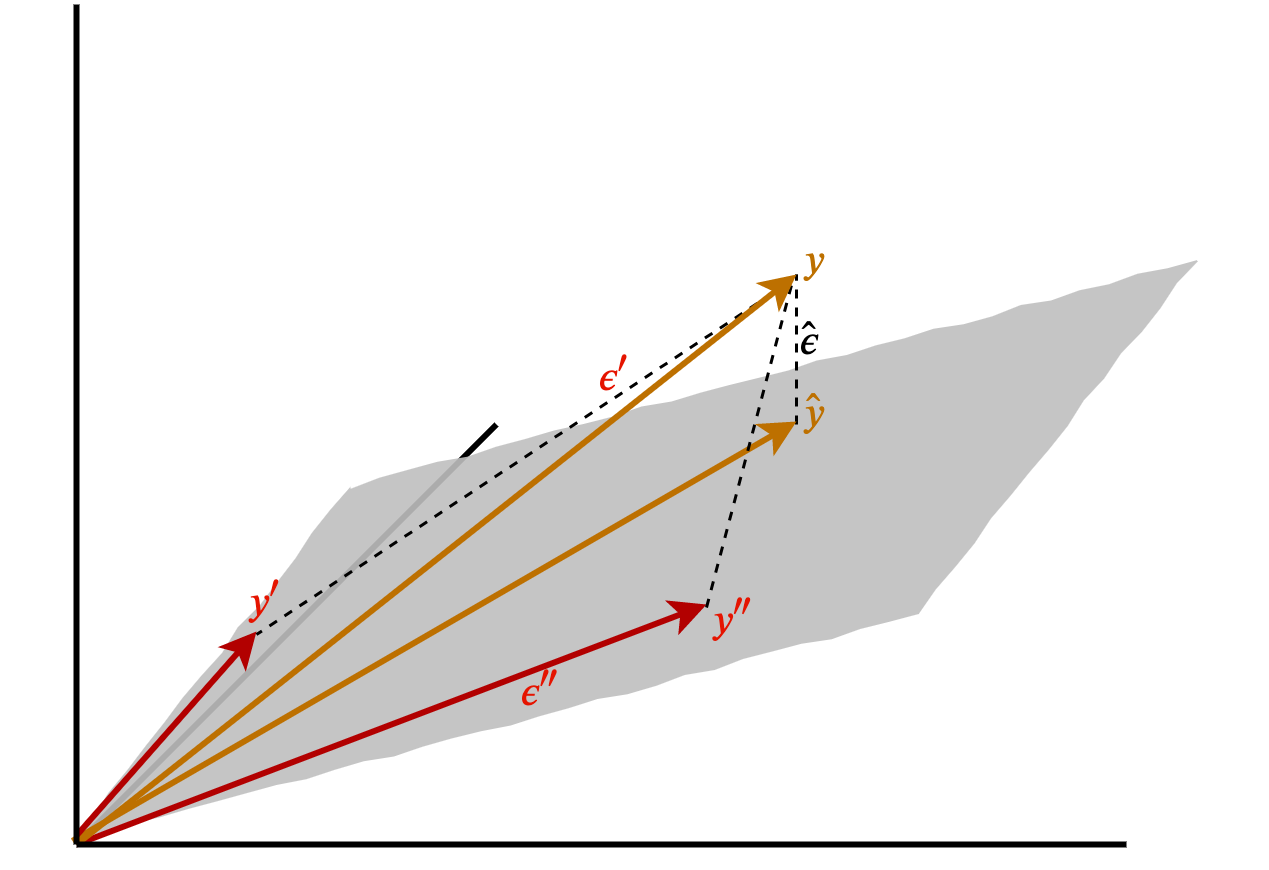
\includegraphics[width=1\linewidth]{images/lp_distances} \caption{Alternative vectors on the column space are further away from y.}\label{fig:lp-distances}
\end{figure}

Hence, linear projection and linear regression can be seen (both algebraically and geometrically) to be solving the same problem -- minimising the (squared) distance between an observed vector \(y\) and prediction vector \(\hat{y}\). This demonstration generalises to many dimensions (observations), though of course it becomes much harder to intuit the geometry of highly-dimensional data. And similarly, with more observations we could also extend the number of predictors too such that \(X\) is not a single column vector but a matrix of predictor variables (i.e.~multivariate regression). Again, visualising what the column space of this matrix would look like geometrically becomes harder.

To summarise, this section has demonstrated two features. First, that linear regression simply is an orthogonal projection. We saw this algebraically by noting that the derivation of OLS coefficients, and subsequently the predicted values from a linear regression, is identical to \(Py\) (where \(P\) is a projection matrix). Second, and geometrically, we intuited why this is the case: namely that projecting onto a lower-dimensional column space involves finding the linear combination of predictors that minimises the Euclidean distance to \(y\), i.e.~\(\hat{y}\). The scalars we use to do so are simply the regression coefficients we would generate using OLS regression.

\hypertarget{wlln}{%
\chapter{Weak Law of Large Numbers and Central Limit Theorem}\label{wlln}}

This chapter focuses on two fundamental theorems that form the basis of our inferences from samples to populations. The Weak Law of Large Numbers (WLLN) provides the basis for generalisation from a sample mean to the population mean. The Central Limit Theorem (CLT) provides the basis for quantifying our uncertainty over this parameter. In both cases, I discuss the theorem itself and provide an annotated proof. Finally, I discuss how the two theorems complement each other.

\hypertarget{weak-law-of-large-numbers}{%
\section{Weak Law of Large Numbers}\label{weak-law-of-large-numbers}}

\hypertarget{theorem-in-plain-english}{%
\subsection{Theorem in Plain English}\label{theorem-in-plain-english}}

Suppose we have a random variable \(X\). From \(X\), we can generate a sequence of random variables \(X_1, X_2,..., X_n\) that are independent and identically distributed (i.i.d.) draws of \(X\). Assuming \(n\) is finite, we can perform calculations on this sequence of random numbers. For example, we can calculate the mean of the sequence \(\bar{X}_n = \frac{1}{n}\sum^n_{i=1}X_i\). This value is the sample mean -- from a much wider population, we have drawn a finite sequence of observations, and calculated the average across them. How do we know that this sample parameter is meaningful with respect to the population, and therefore that we can make inferences from it?

WLLN states that the mean of a sequence of i.i.d. random variables converges in probability to the expected value of the random variable as the length of that sequence tends to infinity. By `converging in probability', we mean that the probability that the difference between the mean of the sample and the expected value of the random variable tends to zero.

In short, WLLN guarantees that with a large enough sample size the sample mean should approximately match the true population parameter. Clearly, this is powerful theorem for any statistical exercise: given we are (always) constrained by a finite sample, WLLN ensures that we can infer from the data something meaningful about the population. For example, from a large enough sample of voters we can estimate the average support for a candidate or party.

More formally, we can state WLLN as follows:

\begin{equation}
\bar{X}_n \xrightarrow{p} \mathbb{E}[X],
\end{equation}

where \(\xrightarrow{p}\) denotes `converging in probability'.

\hypertarget{proof_wlln}{%
\subsection{Proof}\label{proof_wlln}}

To prove WLLN, we use Chebyshev's Inequality (CI). More specifically we first have to prove Chebyshev's Inequality of the Sample Mean (CISM), and then use CISM to prove WLLN. The following steps are based on the proof provided in \citet{aronow2019foundations}.

\textbf{Proof of Chebyshev's Inequality of the Sample Mean.} Chebyshev's Inequality for the Sample Mean (CISM) states that:

\begin{equation}
 P(|\bar{X}_n-\mathbb{E}[X]| \geq k) \leq \frac{var(X)}{k^2 n},
\end{equation}

where \(\bar{X}_n\) is the sample mean of a sequensce of \(n\) independent draws from a random variable \(X\). Recall CI states that \(P(|(X-\mu)/\sigma| \geq k) \leq \frac{1}{k^2}\). To help prove CISM, we can rearrange the left hand side of the inequality by multiplying both sides of the inequality within the probability function by \(\sigma\), such that:

\begin{equation}
   P(|(X-\mu)| \geq k \sigma) \leq \frac{1}{k^2}.
\end{equation}

Then, finally, let us define \(k' = \frac{k}{\sigma}\). Hence:

\begin{align}
  P(|(\bar{X}-\mathbb{E}[X])| \geq k) &= P(|(\bar{X}-\mathbb{E}[X])| \geq k'\sigma) \\
  &\leq \frac{1}{{k'}^2} \\
  &\leq \frac{\sigma^2}{k^2} \\ 
  &\leq \frac{var(\bar{X})}{k^2} \\
  &\leq \frac{var(X)}{k^2 n} \; \; \; \square
\end{align}

This proof is reasonably straightfoward. Using our definition of \(k'\) allows us to us rearrange the probability within CISM to match the form of the Chebyshev Inequality stated above, which then allows us to infer the bounds of the probability. We then replace \(k'\) with \(\frac{k}{\sigma}\), expand and simplify. The move made between the penultimate and final line relies on the fact that variance of the sample mean is equal to the variance in the random variable divided by the sample size (n).\footnote{See Aronow and Miller 2019, p.98.}

\textbf{Applying CISM to WLLN proof.} Given that all probabilities are non-negative and CISM, we can now write:

\begin{equation}
  0 \leq P(|\bar{X}_n−\mathbb{E}[X]| \geq k) \leq \frac{var(X)}{k^2n}. \label{eq:multi_ineq}
\end{equation}

Note that for the first and third term of this multiple inequality, as \(n\) approaches infinity both terms approach 0. In the case of the constant zero, this is trivial. In the final term, note that \(var(X)\) denotes the inherent variance of the random variable, and therefore is constant as \(n\) increases. Therefore, as the denominator increases, the term converges to zero.

Since the middle term is sandwiched in between these two limits, by definition we know that this term must also converge to zero.\footnote{To see why this is the case, given the limits of the first and third terms, Equation \ref{multi_ineq} is of the form $0 \leq A \leq 0$ as $n \to \infty$. The only value of $A$ that satisfies this inequality is 0.} Therefore:

\begin{equation}
\text{lim}_{n \to \infty} P(|\bar{X}_{n}−\mathbb{E}[X]| \geq k) = 0 \; \; \; \square
\end{equation}

Hence, WLLN is proved: for any value of \(k\), the probability that the difference between the sample mean and the expected value is greater or equal to \(k\) converges on zero. Since \(k\)'s value is arbitrary, it can be set to something infinitesimally small, such that the sample mean and expected value converge in value.

\hypertarget{clt}{%
\section{Central Limit Theorem}\label{clt}}

WLLN applies to the value of the statistic itself (the mean value). Given a \emph{single}, n-length sequence drawn from a random variable, we know that the mean of this sequence will converge on the expected value of the random variable. But often, we want to think about what happens when we (hypothetically) calculate the mean across \emph{multiple} sequences i.e.~expectations under repeat sampling.

The Central Limit Theorem (CLT) is closely related to the WLLN. Like WLLN, it relies on asymptotic properties of random variables as the sample size increases. CLT, however, lets us make informative claims about the distribution of the sample mean around the true population parameter.

\hypertarget{theorem-in-plain-english-1}{%
\subsection{Theorem in Plain English}\label{theorem-in-plain-english-1}}

CLT states that as the sample size increases, the distribution of sample means converges to a normal distribution. That is, so long as the underlying distribution has a finite variance (bye bye Cauchy!), then irrespective of the underlying distribution of \(X\) the distribution of sample means will be a normal distribution!

In fact, there are multiple types of CLT that apply in a variety of different contexts -- cases including Bernoulli random variables (de Moivre - Laplace), where random variables are independent but do not need to be identically distributed (Lyapunov), and where random variables are vectors in \(\mathbb{R}^k\) space (multivariate CLT).

In what follows, I will discuss a weaker, more basic case of CLT where we assume random variables are scalar, independent, and identically distributed (i.e.~drawn from the same unknown distribution function). In particular, this section proves that the standardized difference between the sample mean and population mean for i.i.d. random variables converges in distribution to the standard normal distribution \(N(0,1)\). This variant of the CLT is called the Lindeberg-Levy CLT, and can be stated as:

\begin{equation}
  \frac{\bar{X}_n - \mu}{\sigma\sqrt{n}} \xrightarrow{d} N(0,1),
\end{equation}

where \(\xrightarrow{d}\) denotes `converging in distribution'.

In general, the CLT is useful because proving that the sample mean is normally distributed allows us to quantify the uncertainty around our parameter estimate. Normal distributions have convenient properties that allow us to calculate the area under any portion of the curve, given just the same mean and standard deviation. We already know by WLLN that the sample mean will (with a sufficiently large sample) approximate the population mean, so we know that the distribution is also centred around the true population mean. By CLT, the dispersion around that point is therefore normal, and to quantify the probable bounds of the point estimate (under the assumption of repeat sampling) requires only an estimate of the variance.

\hypertarget{primer-characteristic-functions}{%
\subsection{Primer: Characteristic Functions}\label{primer-characteristic-functions}}

CLT is harder (and lengthier) to prove than other proofs we've encountered so far -- it relies on showing that the sample mean converges \emph{in distribution} to a known mathematical form that uniquely and fully describes the normal distribution. To do so, we use the idea of a \emph{characteristic functions}, which simply denotes a function that completely defines a probability function.

For example, and we will use this later on, we know that the characteristic function of the normal distribution is \(e^{it\mu-\frac{\sigma^{2}t^{2}}{2}}\). A standard normal distriibution (where \(\mu = 0, \sigma^2 = 1\)) therefore simplifies to \(e^{-\frac{t^{2}}{2}}\).

More generally, we know that for any scalar random variable \(X\), the characteristic function of \(X\) is defined as:

\begin{equation}
\phi_X(t) = \mathbb{E}[e^{itX}],
\end{equation}

where \(t \in \mathbb{R}\) and \(i\) is the imaginary unit. Proving why this is the case is beyond the purview of this section, so unfortunately I will just take it at face value.

We can expand \(e^{itX}\) as an infinite sum, using a Taylor Series, since \(e^x = 1 + x + \frac{x^2}{2!} + \frac{x^3}{3!} + ...\). Hence:

\begin{equation}
\phi_X(t) = \mathbb{E}[1 + itX + \frac{(itX)^2}{2!} + \frac{(itX)^3}{3!} + ... ],
\end{equation}

Note that \(i^2 = -1\), and since the latter terms tend to zero faster than the second order term we can summarise them as \(o(t^2)\) (they are no larger than of order \(t^2\)). Therefore we can rewrite this expression as:

\begin{equation}
\phi_X(t) = \mathbb{E}[1 + itX - \frac{t^2}{2}X^2 + o(t^2)].
\end{equation}

In the case of continuous random variables, the expected value can be expressed as the integral across all space of the expression multiplied by the probability density, such that:

\begin{equation}
\phi_X(t) = \int^{\infty}_{-\infty}[1 + itX - \frac{t^2}{2}X^2 + o(t^2)]f_X dX,
\end{equation}

and this can be simplified to:

\begin{equation}
\phi_X(t) = 1 + it\mathbb{E}[X] - \frac{t^2}{2}\mathbb{E}[X^2] + o(t^2)],
\end{equation}

since \(1 \times f_X = f_X\), the total area under a probability density necessarily sums to 1; \(\int Xf_X dX\) is the definition of the expected value of X, and so by similar logic \(\int X^2f_X dX = \mathbb{E}[X^2]\).

In \href{https://www.youtube.com/watch?v=0oHjbr2_AhQ}{Ben Lambert's video} introducing the CLT proof, he notes that if we assume X has mean 0 and variance 1, the characteristic function of that distribution has some nice properties, namely that it simplifies to:

\begin{equation}
\phi_X(t) = 1 - \frac{t^2}{2} + o(t^2)],
\end{equation}

since \(\mathbb{E}[X] = 0\) cancelling the second term, and \(\mathbb{E}[X^2] \equiv \mathbb{E}[(X-0)^2] = \mathbb{E}[(X-\mu)^2] = var(X) = 1\).

One final piece of characteristic function math that will help finalise the CLT proof is to note that if we define some random variable \(Q_n = \sum_{i=1}^{n}R_i\), where all \(R_i\) are i.i.d., then the characteristic function of \(Q_n\) can be expressed as \(\phi_{Q_n} (t) = [\phi_{R}(t)]^n\). Again, I will not prove this property here.

\hypertarget{proof-of-clt}{%
\subsection{Proof of CLT}\label{proof-of-clt}}

This proof is based in part on Ben Lambert's excellent \href{https://www.youtube.com/channel/UC3tFZR3eL1bDY8CqZDOQh-w}{YouTube series}, as well as \citet{Lemons_Langevin_Gythiel_2002}.

Given the above discussion of a characteristic function, let us assume a sequence of independent and identically distributed (i.i.d.) random variables \({X_1, X_2, ..., X_n}\), each with mean \(\mu\) and finite\footnote{Hence why degenerate distributions like the Cauchy are not covered by CLT.} variance \(\sigma^2\). The sum of these random variables has mean \(n\mu\) (since each random variable has the same mean) and the variance equivalent to \(n\sigma^2\) (because the random variables are i.i.d. we know that \(var(A,B) = var(A)var(B)\)).

Now let's consider the standardized difference between the actual sum of the random variables and the mean. Standardization simply means dividing a parameter estimate by its standard deviation. In particular, we can consider the following standardized random variable:

\begin{equation}
Z_n = \frac{\sum_{i=1}^{n}(X_i - \mu)}{\sigma\sqrt{n}},
\end{equation}

where \(Z_n\), in words, is the standardised difference between the sum of i.i.d. random variables and the expected value of the sequence. Note that we use the known variance in the denominator.

We can simplify this further:

\begin{equation}
Z_n = \sum_{i=1}^{n}\frac{1}{\sqrt{n}}Y_i,
\end{equation}

where we define a new random variable \(Y_i = \frac{X_i - \mu}{\sigma}.\)

\(Y_i\) has some convenient properties. First, since each random variable \(X_i\) in our sample has mean \(\mu\), we know that \(\mathbb{E}[Y_i] = 0\) since \(\mathbb{E}[X_i] = \mu\) and therefore \(\mu - \mu = 0\). Note that this holds irrespective of the distribution and value of \(\mathbb{E}[X_i]\).

The variance of \(Y_i\) is also recoverable. First note three basic features of variance: if \(a\) is a constant, and \(X\) and \(Y\) are random variables, \(var(a) = 0\); \(var(aX) = a^2var(X)\); and from the variance of a sum \(var(X - Y) = var(A)-var(B)\). Therefore:

\begin{align}
var(\frac{1}{\sigma}(X_i - \mu) &= \frac{1}{\sigma^2}var(X_i - \mu) \\
var(X_i - \mu) &= var(X_i) - var(\mu) \\
&= var(X_i).
\end{align}

Hence:

\begin{equation}
var(Y_i) = \frac{var(X_i)}{\sigma^2} = 1,
\end{equation}

since \(var(X_i) = \sigma^2\).

At this stage, the proof is tantalisingly close. While we have not yet fully characterised the distribution of \(Z_n\) or even \(Y_i\), the fact that \(Y_i\) has unit variance and a mean of zero means suggests we are on the right track to proving that this does asymptotically tend in distribution to the standard normal. In fact, recall from the primer on characteristic functions, that Lambert notes for any random variable with unit variance and mean of 0, \(\phi_X(t) = 1 - \frac{t^2}{2} + o(t^2)\). Hence, we can now say that:

\begin{equation}
\phi_{Y_i}(t) = 1 - \frac{t^2}{2} + o(t^2). \label{eq:cf_yi_simple}
\end{equation}

Now let us return to \(Z_n = \sum_{i=1}^{n}\frac{1}{\sqrt{n}}Y_i\) and using the final bit of characteristic function math in the primer, we can express the characteristic function of \(Z_n\) as:

\begin{equation}
\phi_{Z_n} (t) = [\phi_{Y} (\frac{t}{\sqrt{n}})]^n,
\end{equation}

since \(Y_i\) is divided by the square root of the sample size. Given our previously stated expression of the characteristic function of \(Y_i\):

\begin{equation}
\phi_{Z_n} (t) = [1 - \frac{t^2}{2n} + o(t^2)]]^n.
\end{equation}

We can now consider what happens as \(n \to \infty\). By definition, we know that \(o(t^2)\) converges to zero faster than the other terms, so we can safely ignore it. As a result, and noting that \(e^x = \lim(1+\frac{x}{n})^n\):

\begin{equation}
\lim_{n \to \infty}\phi_{Z_n} (t) = e^{-\frac{t^2}{2}}.
\end{equation}

This expression shows that as \(n\) tends to infinity, the characteristic function of \(Z_n\) is the standard normal distribution (as noted in the characteristic function primer). Therefore:

\begin{align}
\lim_{n \to \infty}Z_n &= N(0,1) \\
\lim_{n \to \infty}\frac{\bar{X}_n - \mu}{\sigma\sqrt{n}} &= N(0,1). \; \; \; \square
\end{align}

The last line here simply follows from the definition of \(Z_n\).

\hypertarget{generalising-clt}{%
\subsection{Generalising CLT}\label{generalising-clt}}

From here, it is possible to intuit the more general CLT that the distribution of sampling means is normally distributed around the true mean \(\mu\) with variance \(\frac{\sigma^2}{n}\). Note this is only a pseudo-proof, because as Lambert notes, multiplying through by \(n\) is complicated by the limit operator with respect to \(n\). However, it is useful to see how these two CLT are closely related.

First, we can rearrange the limit expression using known features of the normal distribution:

\begin{align}
\lim_{n \to \infty}Z_n & \xrightarrow{d} N(0,1) \\
\lim_{n \to \infty} \frac{\sum_{i=1}^{n}(X_i) - n\mu}{\sqrt{n\sigma^2}} & \xrightarrow{d} N(0,1) \\
\lim_{n \to \infty} \sum_{i=1}^{n}(X_i) - n\mu & \xrightarrow{d} N(0,n\sigma^2) \\
\lim_{n \to \infty} \sum_{i=1}^{n}(X_i) & \xrightarrow{d} N(n\mu,n\sigma^2),
\end{align}

since \(aN(b,c) = N(ab, a^2c),\) and \(N(d,e) + f = N(d+f, e).\)

At this penultimate step, we know that the sum of i.i.d. random variables is a normal distribution. To see that the sample mean is also normally distributed, we simply divide through by \(n\):

\begin{equation}
\lim_{n \to \infty} \bar{X} = \frac{1}{n}\sum_{i=1}^{n}(X_i) \xrightarrow{d} N(\mu,\frac{\sigma^2}{n}).
\end{equation}

\hypertarget{limitation-of-clt-and-the-importance-of-wlln}{%
\subsection{Limitation of CLT (and the importance of WLLN)}\label{limitation-of-clt-and-the-importance-of-wlln}}

Before ending, it is worth noting that CLT is a claim with respect to repeat sampling from a population (holding \(n\) constant each time). It is not, therefore, a claim that holds with respect to any particular sample draw. We may actually estimate a mean value that, while probable, lies away from the true population parameter (by definition, since the sample means are normally distributed, there is some dispersion). Constructing uncertainty estimates using CLT on this estimate alone does not guarantee that we are in fact capturing \emph{either} the true variance or the true parameter.

That being said, with sufficiently high-N, we know that WLLN guarantees (assuming i.i.d. observations) that our estimate converges on the population mean. WLLN's asymptotics rely only on sufficiently large sample sizes for a \emph{single} sample. Hence, both WLLN and CLT are crucial for valid inference from sampled data. WLLN leads us to expect that our parameter estimate will in fact be centred approximately near the true parameter. Here, CLT can only say that across multiple samples from the population the distribution of sample means is centred on the true parameter. With WLLN in action, however, CLT allows us to make inferential claims about the uncertainty of this converged parameter.

\hypertarget{slutsky}{%
\chapter{Slutsky's Theorem}\label{slutsky}}

\hypertarget{theorem_slutsky}{%
\section{Theorem in plain English}\label{theorem_slutsky}}

Slutsky's Theorem allows us to make claims about the convergence of random variables. It states that a random variable converging to some distribution \(X\), when multiplied by a variable converging in probability on some constant \(a\), converges in distribution to \(a \times X\). Similarly, if you add the two random variables, they converge in distribution to \(a\) plus \(X\). More formally, the theorem states that if \(X_n \xrightarrow{d} X\) and \(A_n \xrightarrow{p}\), where \(a\) is a constant, then:

\begin{enumerate}
\def\labelenumi{\arabic{enumi}.}
\tightlist
\item
  \(X_n + A_n \xrightarrow{d} X + a\)
\item
  \(A_nX_n \xrightarrow{d} aX\)
\end{enumerate}

Note that if \(A_n\) or \(B_n\) do not converge in probability to constants, and instead converge towards some distribution, then Slutsky's Theorem does not hold. More trivially, if \emph{all} variables converge in probability to constants, then \(A_nX_n + B_n \xrightarrow{p} aX+B\).

\hypertarget{coded-demonstration}{%
\section{Coded demonstration}\label{coded-demonstration}}

This theorem is reasonably intuitive. Suppose that the random variable \(X_n\) converges in distribution to a standard normal distribution \(N(0,1)\). For part 1) of the Theorem, note that when we multiply a standard normal by a constant we ``stretch'' the distribution (assuming \(|a|>1\), else we ``compress'' it). Recall from the discussion of the standard normal in \protect\hyperlink{wlln}{Chapter 5} that \(aN(0,1) = N(0,a^2)\). As \(n\) approaches infinity, therefore, by definition \(A_n \xrightarrow{p} a\), and so the degree to which the standard normal is stretched will converge to that constant too. To demonstrate this feature visually, consider the following simulation:

\begin{Shaded}
\begin{Highlighting}[]
\KeywordTok{library}\NormalTok{(ggplot2)}
\KeywordTok{set.seed}\NormalTok{(}\DecValTok{89}\NormalTok{)}
\NormalTok{N <-}\StringTok{ }\KeywordTok{c}\NormalTok{(}\DecValTok{25}\NormalTok{,}\DecValTok{1000}\NormalTok{,}\DecValTok{1000000}\NormalTok{)}

\NormalTok{results <-}\StringTok{ }\KeywordTok{data.frame}\NormalTok{(}\DataTypeTok{n =} \KeywordTok{as.factor}\NormalTok{(}\KeywordTok{levels}\NormalTok{(N)),}
                      \DataTypeTok{X_n =} \KeywordTok{as.numeric}\NormalTok{(),}
                      \DataTypeTok{A_n =} \KeywordTok{as.numeric}\NormalTok{(),}
                      \DataTypeTok{ax =} \KeywordTok{as.numeric}\NormalTok{())}

\ControlFlowTok{for}\NormalTok{ (n }\ControlFlowTok{in}\NormalTok{ N) \{}
\NormalTok{  X_n <-}\StringTok{ }\KeywordTok{rnorm}\NormalTok{(n)}
\NormalTok{  A_n <-}\StringTok{ }\DecValTok{2} \OperatorTok{+}\StringTok{ }\KeywordTok{exp}\NormalTok{(}\OperatorTok{-}\NormalTok{n)}
\NormalTok{  aX <-}\StringTok{ }\NormalTok{A_n }\OperatorTok{*}\StringTok{ }\NormalTok{X_n}
  
\NormalTok{  results <-}\StringTok{ }\KeywordTok{rbind}\NormalTok{(results, }\KeywordTok{cbind}\NormalTok{(n, X_n, A_n, aX))}
  
\NormalTok{\}}

\KeywordTok{ggplot}\NormalTok{(results, }\KeywordTok{aes}\NormalTok{(}\DataTypeTok{x =}\NormalTok{ aX)) }\OperatorTok{+}
\StringTok{  }\KeywordTok{facet_wrap}\NormalTok{(n}\OperatorTok{~}\NormalTok{., }\DataTypeTok{ncol =} \DecValTok{3}\NormalTok{, }\DataTypeTok{labeller =} \StringTok{"label_both"}\NormalTok{) }\OperatorTok{+}
\StringTok{  }\KeywordTok{geom_density}\NormalTok{() }\OperatorTok{+}
\StringTok{  }\KeywordTok{labs}\NormalTok{(}\DataTypeTok{y =} \StringTok{"p(aX)"}\NormalTok{)}
\end{Highlighting}
\end{Shaded}

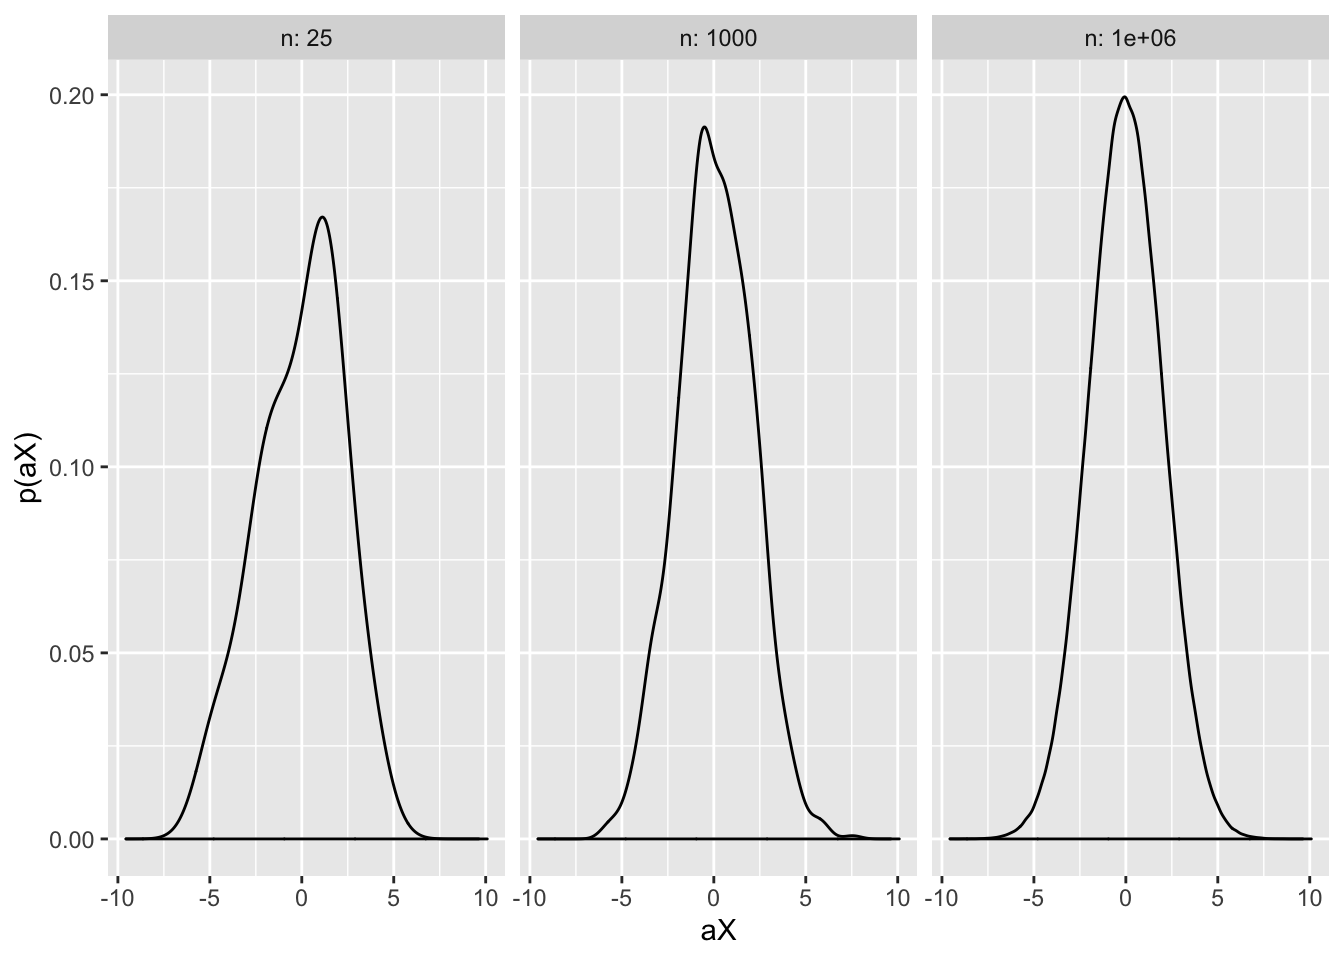
\includegraphics{10EconometricTheorems_files/figure-latex/unnamed-chunk-2-1.pdf}

Here we have defined two random variables: \texttt{X\_n} is a standard normal, and \texttt{A\_n} converges in value to 2. Varying the value of \texttt{n}, I take \(n\) draws from a standard normal distribution and calculate the value the converging constant \(A_n\). I then generate the product of these two variables. The figure plots the resulting distribution \texttt{aX}. We can see that as \texttt{n} increases, the distribution becomes increasingly normal, remains centred around 0 and the variance approaches 4 (since 95\% of the curve is approximately bounded between \(0 \pm 2\times\sqrt{var(aX)} = 0 \pm 2\times2 = 0 \pm 4\)).

Similarly, if we add the constant \(a\) to a standard distribution, the effect is to shift the distribution in its entirety (since a constant has no variance, it does not `'stretch'' the distribution). As \(A_n\) converges in probability, therefore, the shift converges on the constant \(a\). Again, we can demonstrate this result in R:

\begin{Shaded}
\begin{Highlighting}[]
\KeywordTok{library}\NormalTok{(ggplot2)}
\KeywordTok{set.seed}\NormalTok{(}\DecValTok{89}\NormalTok{)}
\NormalTok{N <-}\StringTok{ }\KeywordTok{c}\NormalTok{(}\DecValTok{25}\NormalTok{,}\DecValTok{1000}\NormalTok{,}\DecValTok{1000000}\NormalTok{)}

\NormalTok{results <-}\StringTok{ }\KeywordTok{data.frame}\NormalTok{(}\DataTypeTok{n =} \KeywordTok{as.factor}\NormalTok{(}\KeywordTok{levels}\NormalTok{(N)),}
                      \DataTypeTok{X_n =} \KeywordTok{as.numeric}\NormalTok{(),}
                      \DataTypeTok{A_n =} \KeywordTok{as.numeric}\NormalTok{(),}
                      \DataTypeTok{a_plus_X=} \KeywordTok{as.numeric}\NormalTok{())}

\ControlFlowTok{for}\NormalTok{ (n }\ControlFlowTok{in}\NormalTok{ N) \{}
\NormalTok{  X_n <-}\StringTok{ }\KeywordTok{rnorm}\NormalTok{(n)}
\NormalTok{  A_n <-}\StringTok{ }\DecValTok{2} \OperatorTok{+}\StringTok{ }\KeywordTok{exp}\NormalTok{(}\OperatorTok{-}\NormalTok{n)}
\NormalTok{  a_plus_X <-}\StringTok{ }\NormalTok{A_n }\OperatorTok{+}\StringTok{ }\NormalTok{X_n}
  
\NormalTok{  results <-}\StringTok{ }\KeywordTok{rbind}\NormalTok{(results, }\KeywordTok{cbind}\NormalTok{(n, X_n, A_n, a_plus_X))}
  
\NormalTok{\}}

\KeywordTok{ggplot}\NormalTok{(results, }\KeywordTok{aes}\NormalTok{(}\DataTypeTok{x =}\NormalTok{ a_plus_X)) }\OperatorTok{+}
\StringTok{  }\KeywordTok{facet_wrap}\NormalTok{(n}\OperatorTok{~}\NormalTok{., }\DataTypeTok{ncol =} \DecValTok{3}\NormalTok{, }\DataTypeTok{labeller =} \StringTok{"label_both"}\NormalTok{) }\OperatorTok{+}
\StringTok{  }\KeywordTok{geom_density}\NormalTok{() }\OperatorTok{+}
\StringTok{  }\KeywordTok{geom_vline}\NormalTok{(}\DataTypeTok{xintercept =} \DecValTok{2}\NormalTok{, }\DataTypeTok{linetype =} \StringTok{"dashed"}\NormalTok{) }\OperatorTok{+}
\StringTok{  }\KeywordTok{labs}\NormalTok{(}\DataTypeTok{y =} \StringTok{"p(a+X)"}\NormalTok{, }\DataTypeTok{x=}\StringTok{"a+X"}\NormalTok{)}
\end{Highlighting}
\end{Shaded}

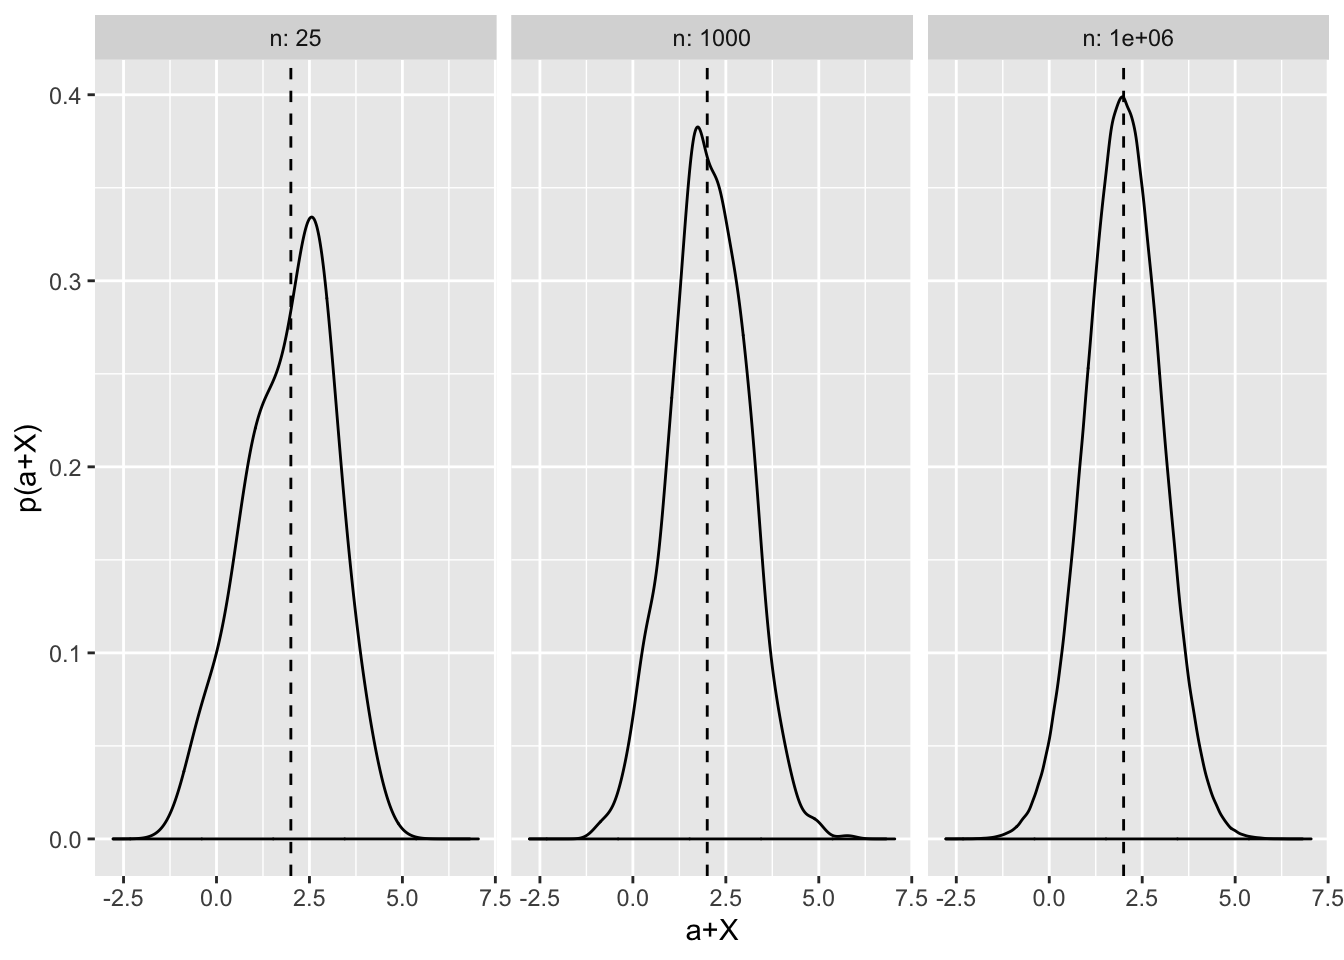
\includegraphics{10EconometricTheorems_files/figure-latex/unnamed-chunk-3-1.pdf}

As \texttt{n} becomes larger, the resulting distribution becomes approximately normal, with variance of 1 and a mean value centred around \(0 + a = 2\).

Slutsky's Theorem is so useful precisely because it allows us to combine multiple random variables with known asymptotics, and retain this knowledge i.e.~we know what the resultant distribution will converge to assuming \(n \to \infty\).

\hypertarget{proof-of-slutskys-theorem}{%
\section{Proof of Slutsky's Theorem}\label{proof-of-slutskys-theorem}}

Despite the intuitive appeal of Slutsky's Theorem, the proof is less straightforward. It relies on the continuous mapping theorem (CMT), which in turns rests on several other theorems such as the Portmanteau Theorem. To avoid the rabbit hole of proving all necessary antecedent theorems, I simply introduce and state the continuous mapping theorem (CMT) here, and then show how this can be used to prove Slutsky's Theorem.

\hypertarget{cmt}{%
\subsection{CMT}\label{cmt}}

The continuous mapping theorem states that if there is some random variable such that \(X_n \xrightarrow{d} X\), then \(g(X_n) \xrightarrow{d} g(X)\), so long as \(g\) is a continuous function. In approximate terms (which are adequate for our purpose), a continuous function is one in which for a given domain the function can be represented as an single unbroken curve (or hyperplane in many dimensions). For example, consider the graph of \(f(x) = x^{-1}\). For the domain \(D_{+}: \mathbb{R} > 0\), this function is continuous. But for the domain \(D_{\infty}: \mathbb{R}\), the function is discontinuous because the function is undefined when \(x = 0\).

In short, CMT states that a continuous function preserves the asymptotic limits of a random variable. More broadly (and again, I do not prove this here), CMT entails that \(g(P_n,Q_n,...,Z_n) \xrightarrow{d} g(P,Q,...,Z)\) if all \(P_n, Q_n,...\) etc. converge in distribution to \(P,Q,...\) respectively.

\hypertarget{proof-using-cmt}{%
\subsection{Proof using CMT}\label{proof-using-cmt}}

How does this help prove Slutsky's Theorem? We know by the definitions in Slutsky's Theorem that \(X_n \xrightarrow{d} X\) and, by a similar logic, we know that \(A_n \xrightarrow{d} a\) (since \(A_n \xrightarrow{p} a\), and converging in probability entails converging in distribution). So we can note that the joint vector \((X_n, A_n) \xrightarrow{d} (X,a)\). By CMT, therefore, \(g(X_n, A_n) \xrightarrow{d} g(X,a)\). Hence, any continuous function \(g\) will preserve the limits of the respective distributions.

Given this result, it is sufficient to note that both addition and multiplication are continuous functions. Again, I do not show this here but the continuity of addition and multiplication (both scalar and vector) can be proved mathematically (for example see one such proof \href{http://mathonline.wikidot.com/continuity-of-addition-scalar-multiplication-and-multiplicat\%5D.}{here} For an intuitive explanation, think about the diagonal line \(y=X\) -- any multiplication of that line is still a single, uninterrupted line (\(y = aX\)) assuming \(a\) is a constant. Similarly, adding a constant to the function of a line also yields an uninterrupted line (e.g.~\(y= X + a\)).

Hence, CMT guarantees both parts 1 and 2 of the Theorem. \(\square\)

\hypertarget{applications_slutsky}{%
\section{Applications}\label{applications_slutsky}}

Slutsky's Theorem is a workhorse theorem that allows researchers to make claims about the limiting distributions of multiple random variables. Instead of being used in applied settings, it typically underpins the modelling strategies used in applied research. For example, \citet{aronow_representative2015} consider the problem of weighting multiple regression when the data sample is unrepresentative of the population of interest. In their proofs, they apply Slutsky's Theorem at two different points to prove that their weighted regression estimates converge in probability on the weighted expectation of individual treatment effects, and subsequently, that the same coefficient converges in probability to the true average treatment effect in the population.

\hypertarget{proving-the-consistency-of-sample-variance-and-the-normality-of-the-t-statistic}{%
\subsection{Proving the consistency of sample variance, and the normality of the t-statistic}\label{proving-the-consistency-of-sample-variance-and-the-normality-of-the-t-statistic}}

In the remainder of this chapter, I consider applications of both Central Mapping Theorem and Slutsky's Theorem in fundamental statistical proofs. I first show how CMT can be used to prove the consistency of the variance of a random variable, and subsequently how in combination with Slutsky's Theorem this helps prove the normality of a t-statistic. These examples are developed from \href{http://personal.psu.edu/drh20/asymp/lectures/asymp.pdf}{David Hunter's notes} on asymptotic theory that accompany his Penn State course in large-sample theory.

\hypertarget{consistency-of-the-sample-variance-estimator}{%
\subsubsection{Consistency of the sample variance estimator}\label{consistency-of-the-sample-variance-estimator}}

First, let us define the sample variance (\(s^2_n\)) of a sequence of i.i.d random variables drawn from a distribution \(X\) with \(\mathbb{E}[X] = \mu\) and \(var(X) = \sigma^2\) as:

\[ s^2_n = \frac{1}{n-1}\sum_{i=1}^n (X_i - \bar{X_n})^2.\]

We can show that the sample variance formula above is a consistent estimator of the true variance \(\sigma^2\). That is, as the sequence of i.i.d. random variables \(X_1, X_2,...\) increases in length, the sample variance estimator of that sequence converges in probability to the true variance value \(\sigma^2\).

We can prove this by redefining \(s^2\) as follows:

\[ s^2_n = \frac{n}{n-1} \left[\frac{1}{n}\sum_{i=1}^n(X_i - \mu)^2 - (\bar{X_n}-\mu)^2 \right], \]
which clearly simplifies to the conventional definition of \(s^2\) as first introduced.

From here, we can note using WLLN, that \((\bar{X_n} - \mu) \xrightarrow{p} 0\), and hence that \((\bar{X_n}-\mu)^2 \xrightarrow{p} 0\). Note that this term converges in probability to a constant. Moreover, \(\frac{1}{n}\sum_{i=1}^n(X_i - \mu)^2 \xrightarrow{p} \mathbb{E}[X_i - \mu] = var(X) = \sigma^2\), by definition.

Now let us define an arbitrary continuous function \(g(A_n,B_n)\). We know by CMT that if \(A_n \xrightarrow{p} A, B_n \xrightarrow{p} B\) then \(g(A_n, B_n) \xrightarrow{p} g(A,B)\). And hence, using the implications above we know that for any continuous function \(g\) that \(g(\frac{1}{n}\sum_{i=1}^n(X_i - \mu)^2, (\bar{X_n} - \mu)) \xrightarrow{p} g(\sigma^2,0)\).

Since subtraction is a continuous function, we therefore know that:

\[ \left[\frac{1}{n}\sum_{i=1}^n(X_i - \mu)^2 - (\bar{X_n}-\mu)^2\right] \xrightarrow{p} \left[\sigma^2 - 0\right] = \sigma^2.\]

Separately we can intuitively see that \(\frac{n}{n-1} \xrightarrow{p} 1.\) Hence, by applying CMT again to this converging variable multiplied by the converging limit of the above (since multiplication is a continuous function), we can see that:

\[ s^2_n \xrightarrow{p} 1 \times \sigma^2 = \sigma^2 \;\;\; \square\]

\hypertarget{normality-of-the-t-statistic}{%
\subsubsection{Normality of the t-statistic}\label{normality-of-the-t-statistic}}

Let's define a t-statistic as:

\[ t_n = \frac{\sqrt{n}(\bar{X}_n-\mu)}{\sqrt{\hat{\sigma^2}}}\]

By the Central Limit Theorem (CLT, \protect\hyperlink{wlln}{Chapter 5}), we know that for a random variable \(X\) with mean \(\mu\) and variance \(\sigma^2\) that \(\sqrt{n}(\bar{X}_n - \mu) \xrightarrow{d} N(0,\sigma^2)\).

We also know from the proof above that if \(\hat{\sigma}^2 = s^2\) then \(\hat{\sigma}^2 \xrightarrow{p} \sigma^2\) -- a constant. Given this, we can also note that \(\frac{1}{\hat{\sigma^2}} \xrightarrow{p} \frac{1}{\sigma^2}\).

Hence, by Slutsky's Theorem:

\begin{align}
\sqrt{n}(\bar{X}_n-\mu) \times \frac{1}{\sqrt{\sigma^2}} &\xrightarrow{d} N(0,\sigma^2) \times \frac{1}{\sqrt{\sigma^2}} \\
&= \sigma N(0,1) \times \frac{1}{\sigma}\\
&= N(0,1) \;\;\; \square
\end{align}

One brief aspect of this proof that is noteworthy is that since Slutsky's Theorem rests on the CMT, the application of Slutsky's Theorem requires that the function of the variables \(g\) (in this case multiplication) is continuous and defined for the specified domain. Note that \(\frac{1}{0}\) is undefined and therefore that the above proof only holds when we assume \(\sigma^2 > 0\). Hence why in many statistics textbooks and discussions of model asymptotics, authors note that they must assume a positive, non-zero variance.

\hypertarget{big-op-and-little-op}{%
\chapter{Big Op and little op}\label{big-op-and-little-op}}

\hypertarget{stochastic-order-notation}{%
\section{Stochastic order notation}\label{stochastic-order-notation}}

\textbf{``Big Op''} (\emph{big oh-pee}), or in algebraic terms \(O_p\), is a shorthand means of characterising the convergence in probability of a set of random variables. It directly builds on the same sort of convergence ideas that were discussed in Chapters \protect\hyperlink{wlln}{5} and \protect\hyperlink{slutsky}{6}.

Big Op means that some given random variable is stochastically bounded. If we have some random variable \(X_n\) and some constant \(a_n\) (where n indexes both sets), then

\[ X_n = O_p(a_n)\] is the same as saying that \[ P(|\frac{X_n}{a_n}| > \delta) < \epsilon, \forall n > N. \]
\(M \text{ and } N\) here are just finite numbers, and \(\epsilon\) is some arbitrary (small) number. In plain English, \(O_p\) means that for a large enough \(n\) there is some number (\(M\)) such that the probability that the random variable \(\frac{X_n}{a_n}\) is larger than that number is essentially zero. It is ``bounded in probability'' \citep[Section 2.2]{vaart_1998}.

\textbf{``Little op''} (\emph{litle oh-pee}), or \(o_p\), refers to convergence in probability towards zero. \(X_n = o_p(1)\) is the same as saying

\[ \lim_{n\to\infty} (P|X_n| \geq \epsilon) = 0, \forall\epsilon > 0. \]

By definition of the notation, if \(X_n = o_p(a_n)\) then

\[ \frac{x_n}{a_n} = o_p(1).\]

In turn, we can therefore express \(X_n = o_p(a_n)\) as

\[ \lim_{n\to\infty} (P|\frac{X_n}{a_n}| \geq \epsilon) = 0, \forall\epsilon > 0.\]
In other words, \(X_n = o_p(a_n)\) if and only if \(\frac{X_n}{a_n} \xrightarrow{p} 0\).

\hypertarget{relationship-of-big-o-and-little-o}{%
\subsection{Relationship of big-O and little-o}\label{relationship-of-big-o-and-little-o}}

\(O_p\) and \(o_p\) may seem quite similar, and that's because they are! Another way to express \(X_n = O_p(a_n)\), is

\[\forall \epsilon\;\; \exists N_\epsilon,\delta_\epsilon \;\; s.t. \forall n > N_\epsilon,\;\; P(|\frac{X_n}{a_n}| \geq \delta_\epsilon) \leq \epsilon.\]
This restatement makes it clear that the values of \(\delta\) and \(N\) are to be found with respect to \(\epsilon\). That is, we only have to find one value of \(N\) and \(\delta\) for each \(epsilon\), and these can differ across \(\epsilon\)'s.

Using the same notation, \(X_n = o_p(a_n)\) can be expressed as

\[\forall \epsilon,\delta\;\; \exists N_{\epsilon,\delta} \;\; s.t. \forall n > N_{\epsilon,\delta},\;\; P(|\frac{X_n}{a_n}| \geq \delta) \leq \epsilon.\]
\(o_p\) is therefore a more general statement, ranging over all values of \(\epsilon\) \emph{and} \(\delta\), and hence any combination of those two values. In other words, for any given pair of values for \(\epsilon\) and \(\delta\) there must be some \(N\) that satisfies the above inequality (assuming \(X_n = o_p(a_n)\)).

Note also, therefore that \(o_p(a_n)\) entails \(O_p(a_n)\), but that the inverse is not true. If for all \(\epsilon\) and \(\delta\) there is some \(N_{\epsilon,\delta}\) that satisfies the inequality, then it must be the case that for all \(\epsilon\) there exists some \(\delta\) such that the inequality also holds. But just because for some \(\delta_\epsilon\) the inequality holds, this does not mean that it will hold for \emph{all} \(\delta\).

\hypertarget{notational-shorthand-and-arithmetic-properties}{%
\section{Notational shorthand and ``arithmetic" properties}\label{notational-shorthand-and-arithmetic-properties}}

Expressions like \(X_n = o_p\left(\frac{1}{\sqrt{n}}\right)\) do not contain literal identities. Big and little o are merely shorthand ways of expressing how some random variable converges (either to a bound or zero). Suppose for instance that we know \(X_n = o_p(\frac{1}{n})\). We also therefore know that \(X_n = o_p(\frac{1}{n^{0.5}})\). Analogously, think about an object accelerating at a rate of at least \(10ms^{-2}\) -- that car is also accelerating at a rate at least \(5ms^{-2}\). But it's not the case that \(o_p(\frac{1}{n}) = o_p(\frac{1}{\sqrt{n}})\). For instance a car accelerating at least as fast as \(5ms^{-2}\) is not necessarily accelerating at least as fast as \(10ms^{-2}\).

Hence, when we use stochastic order notation we should be careful to think of it as implying something rather than making the claim that some random variable or expression involving random variables \emph{equals} some stochastic order.

That being said, we can note some simple implications of combining \(O_p\) and/or \(o_p\) terms, including:

\begin{itemize}
\item
  \(o_p(1) + o_p(1) = o_p(1)\) -- this is straightforward: two terms that both converge to zero at the same rate, collectively converge to zero at that rate. Note this is actually just an application of \protect\hyperlink{cmt}{Continuous Mapping Theorem}, since If \(X_n = o_p(1), Y_n = o_p(1)\) then \(X_n \xrightarrow{p} 0, Y_n \xrightarrow{p} 0\) then the addition of these two terms is a continuous mapping function, and therefore \(X_n + Y_n \xrightarrow{p} 0, \; \therefore X_n+Y_n = o_p(1)\).
\item
  \(O_p(1) + o_p(1) = O_p(1)\) -- a term that is bounded in probability (\(O_p(1)\)) plus a term converging in probability to zero, is bounded in probability.
\item
  \(O_p(1)o_p(1) = o_p(1)\) -- a bounded probability multiplied by a term that converges (in the same order) to zero itself converges to zero.
\item
  \(o_p(R) = R\times o_p(1)\) -- again this is easy to see, since suppose \(X_n = o_p(R)\), then \(X_n/R = o_p(1)\), and so \(X_n = Ro_p(1)\).
\end{itemize}

Further rules, and intuitive explanations for their validity, can be found in Section 2.2 of \citet{vaart_1998}. The last rule above, however, is worth dwelling on briefly since it makes clear why we use different rate terms (\(R\)) in the little-o operator. Consider two rates \(R^{(1)} = \frac{1}{\sqrt{n}}\), \(R^{(2)} = \frac{1}{\sqrt[3]{2}}\), and some random variable \(Y_n \xrightarrow{p}0\), that is \(Y_n = o_p(1)\). Given the final rule (and remembering the equals signs should not be read literally), if \(X_n^{(1)} = o_p(R^{(1)})\), then

\[
X_n^{(1)} = \frac{1}{\sqrt{n}}\times Y_n,
\]
and if \(X_n^{(2)} = o_p(R^{(2)})\), then

\[
X_n^{(2)} = \frac{1}{\sqrt[3]{n}} \times Y_n.
\]
For each value of \(Y_n\) as \(n\) approaches infinity, \(X_n^{(1)}\) is smaller \(X_n^{(2)}\). In other words, \(X_n^{(2)}\) will converge in probably towards zero more slowly. This implication of the notation, again,

\hypertarget{why-is-this-usefulfn_cite1}{%
\section[Why is this useful?]{\texorpdfstring{Why is this useful?\footnote{The first two examples in this section are adapted from Ashesh Rambachan's \href{https://scholar.harvard.edu/files/asheshr/files/asymptotics-slides.pdf}{Asymptotics Review lecture slides}, from Harvard Math Camp -- Econometrics 2018.}}{Why is this useful?}}\label{why-is-this-usefulfn_cite1}}

A simple (trivial) example of this notation is to consider a sequence of random variables \(X_n\) with known \(\mathbb{E}[X_n] = X\). We can therefore decompose \(X_n = X + o_p(1)\), since we know by the \protect\hyperlink{wlln}{Weak Law of Large Numbers} that \(X_n \xrightarrow{p} X\). This is useful because, without having to introduce explicit limits into our equations, we know that with a sufficiently large \(n\), the second term of our decomposition converges to zero, and therefore we can (in a hand-wavey fashion) ignore it.

Let's consider a more meaningful example. Suppose now that \(X_n \sim N(0,n)\). Using known features of normal distributions, we can rearrange this to

\[ \frac{X_n}{\sqrt{n}} \sim N(0,1). \]
There exists some \(M\) such that the probability that a value from \(N(0,1)\) exceeds \(M\) is less than \(\epsilon > 0\), and therefore

\[ X_n = O_p(\sqrt{n}).\]

\(X_n\) is also little-op of \(n\) since

\[\begin{aligned}
\frac{X_n}{n} &\sim N(0,\frac{n}{n^2})\\
&\sim N(0,\frac{1}{n})\\
\end{aligned}\]

And so we just need to prove the righthand side above is \(o_p(1)\). To do so note that:

\[\begin{aligned}
P(|N(0,\frac{1}{n})|> \epsilon) &= P(\frac{1}{\sqrt{n}}|N(0,1)| > \epsilon )\\
&= P(|N(0,1)| > \sqrt{n}\epsilon) \xrightarrow{p} 0.
\end{aligned}\]

The last follows since \(\sqrt{n} \to \infty\), and so the probability that the standard normal is greater than \(\infty\) decreases to zero. Hence \(X_n = o_p(n)\).

\[ \lim_{n\to\infty}P\left( \left| \frac{N(0,\frac{1}{n})}{n} \right| \geq \epsilon \right) = 0 = o_p(1), \]

for all \(\epsilon > 0\), and therefore that

\[X_n = o_p(n)\].

The big-O, little-o notation captures the complexity of the equation or, equivalently, the rate at which it converges. One way to read \(X_n = o_p(a_n)\) is that, for any multiple of \(j\), \(X_n\) converges in probability to zero at the rate determined by \(a_n\). So, for example, \(o_p(a_n^2)\) converges faster than \(o_p(a_n)\), since for some random variable \(X_n\), \(\frac{X_n}{a_n^2} < \frac{X_n}{a_n}, n > 1.\)

When we want to work out the asymptotic limits of a more complicated equation, where multiple terms are affected by the number of observations, if we have a term that converges in probability to zero at a faster rate than others then we can safely ignore that term.

\hypertarget{estimator_consistency}{%
\section{Worked Example: Consistency of mean estimators}\label{estimator_consistency}}

A parameter is ``consistent'' if it converges in probability to the true parameter as the number of observations increases. More formally, a parameter estimate \(\hat{\theta}\) is consistent if

\[ P(|\hat{\theta} - \theta| \geq \epsilon) \xrightarrow{p} 0, \]
where \(\theta\) is the true parameter.

One question we can ask is how \emph{fast} our consistent parameter estimate converges on the true parameter value. This is an ``applied'' methods problem to the extent that, as researchers seeking to make an inference about the true parameter, and confronted with potentially many ways of estimating it, we want to choose an efficient estimator i.e.~one that gets to the truth quickest!

Let's suppose we want to estimate the population mean of \(X\), i.e.~\(\bar{X}\). Suppose further we have two potential estimators, the sample mean is \(\frac{1}{N}\sum_{i=1}^N X_i\) and the median is \(X_{(N+1)/2}\), where \(N = 2n + 1\) (we'll assume an odd number of observations for the ease of calculation) and \(X\) is an ordered sequence from smallest to largest.

We know by the \protect\hyperlink{clt}{Central Limit Theorem} that the sample mean

\[ \bar{X}_N \sim \mathcal{N}(\theta, \frac{\sigma^2}{N}), \]

and note that I use \(\mathcal{N}\) to denote the normal distribution function, to avoid confusion with the total number of observations \(N\).

Withholding the proof, the large-sample distribution of the median estimator can be expressed \emph{approximately}\footnote{See \href{https://mathworld.wolfram.com/StatisticalMedian.html}{this Wolfram MathWorld post} for more information about the exact CLT distribution of sample medians.} as

\[ \text{Med}(X_1,X_2,...,X_N) \sim \mathcal{N}(\theta, \frac{\pi\sigma^2}{2N}). \]

How do these estimators perform in practice? Let's first check this via Monte Carlo, by simulating draws of a standard normal distribution with various sizes of N and plotting the resulting distribution of the two estimators:

\begin{Shaded}
\begin{Highlighting}[]
\KeywordTok{library}\NormalTok{(tidyverse)}
\KeywordTok{library}\NormalTok{(ccaPP) }\CommentTok{# This pkg includes a fast algorithm for the median}
\end{Highlighting}
\end{Shaded}

\begin{Shaded}
\begin{Highlighting}[]
\CommentTok{# Compute sample mean and median 1000 times, using N draws from std. normal}
\NormalTok{rep_sample <-}\StringTok{ }\ControlFlowTok{function}\NormalTok{(N) \{}
\NormalTok{  sample_means <-}\StringTok{ }\KeywordTok{c}\NormalTok{()}
\NormalTok{  sample_medians <-}\StringTok{ }\KeywordTok{c}\NormalTok{()}
  \ControlFlowTok{for}\NormalTok{ (s }\ControlFlowTok{in} \DecValTok{1}\OperatorTok{:}\DecValTok{1000}\NormalTok{) \{}
\NormalTok{    sample <-}\StringTok{ }\KeywordTok{rnorm}\NormalTok{(N)}
\NormalTok{    sample_means[s] <-}\StringTok{ }\KeywordTok{mean}\NormalTok{(sample)}
\NormalTok{    sample_medians[s] <-}\StringTok{ }\KeywordTok{fastMedian}\NormalTok{(sample)}
\NormalTok{  \}}
  \KeywordTok{return}\NormalTok{(}\KeywordTok{data.frame}\NormalTok{(}\DataTypeTok{N =}\NormalTok{ N, }\DataTypeTok{Mean =}\NormalTok{ sample_means, }\DataTypeTok{Median =}\NormalTok{ sample_medians))}
\NormalTok{\}}

\KeywordTok{set.seed}\NormalTok{(}\DecValTok{89}\NormalTok{)}
\NormalTok{Ns <-}\StringTok{ }\KeywordTok{c}\NormalTok{(}\DecValTok{5}\NormalTok{,}\KeywordTok{seq}\NormalTok{(}\DecValTok{50}\NormalTok{,}\DecValTok{250}\NormalTok{, }\DataTypeTok{by =} \DecValTok{50}\NormalTok{)) }\CommentTok{# A series of sample sizes}

\CommentTok{# Apply function and collect results, then pivot dataset to make plotting easier}
\NormalTok{sim_results <-}\StringTok{ }\KeywordTok{do.call}\NormalTok{(}\StringTok{"rbind"}\NormalTok{, }\KeywordTok{lapply}\NormalTok{(Ns, }\DataTypeTok{FUN =} \ControlFlowTok{function}\NormalTok{(x) }\KeywordTok{rep_sample}\NormalTok{(x))) }\OperatorTok\StringTok{ }
\StringTok{  }\KeywordTok{pivot_longer}\NormalTok{(}\OperatorTok{-}\NormalTok{N, }\DataTypeTok{names_to =} \StringTok{"Estimator"}\NormalTok{, }\DataTypeTok{values_to =} \StringTok{"estimate"}\NormalTok{)}

\KeywordTok{ggplot}\NormalTok{(sim_results, }\KeywordTok{aes}\NormalTok{(}\DataTypeTok{x =}\NormalTok{ estimate, }\DataTypeTok{color =}\NormalTok{ Estimator, }\DataTypeTok{fill =}\NormalTok{ Estimator)) }\OperatorTok{+}
\StringTok{  }\KeywordTok{facet_wrap}\NormalTok{(}\OperatorTok{~}\NormalTok{N, }\DataTypeTok{ncol =} \DecValTok{2}\NormalTok{, }\DataTypeTok{scales =} \StringTok{"free_y"}\NormalTok{, }\DataTypeTok{labeller =} \StringTok{"label_both"}\NormalTok{) }\OperatorTok{+}
\StringTok{  }\KeywordTok{geom_density}\NormalTok{(}\DataTypeTok{alpha =} \FloatTok{0.5}\NormalTok{) }\OperatorTok{+}
\StringTok{  }\KeywordTok{labs}\NormalTok{(}\DataTypeTok{x =} \StringTok{"Value"}\NormalTok{, }\DataTypeTok{y =} \StringTok{"Density"}\NormalTok{) }\OperatorTok{+}
\StringTok{  }\KeywordTok{theme}\NormalTok{(}\DataTypeTok{legend.position =} \StringTok{"bottom"}\NormalTok{)}
\end{Highlighting}
\end{Shaded}

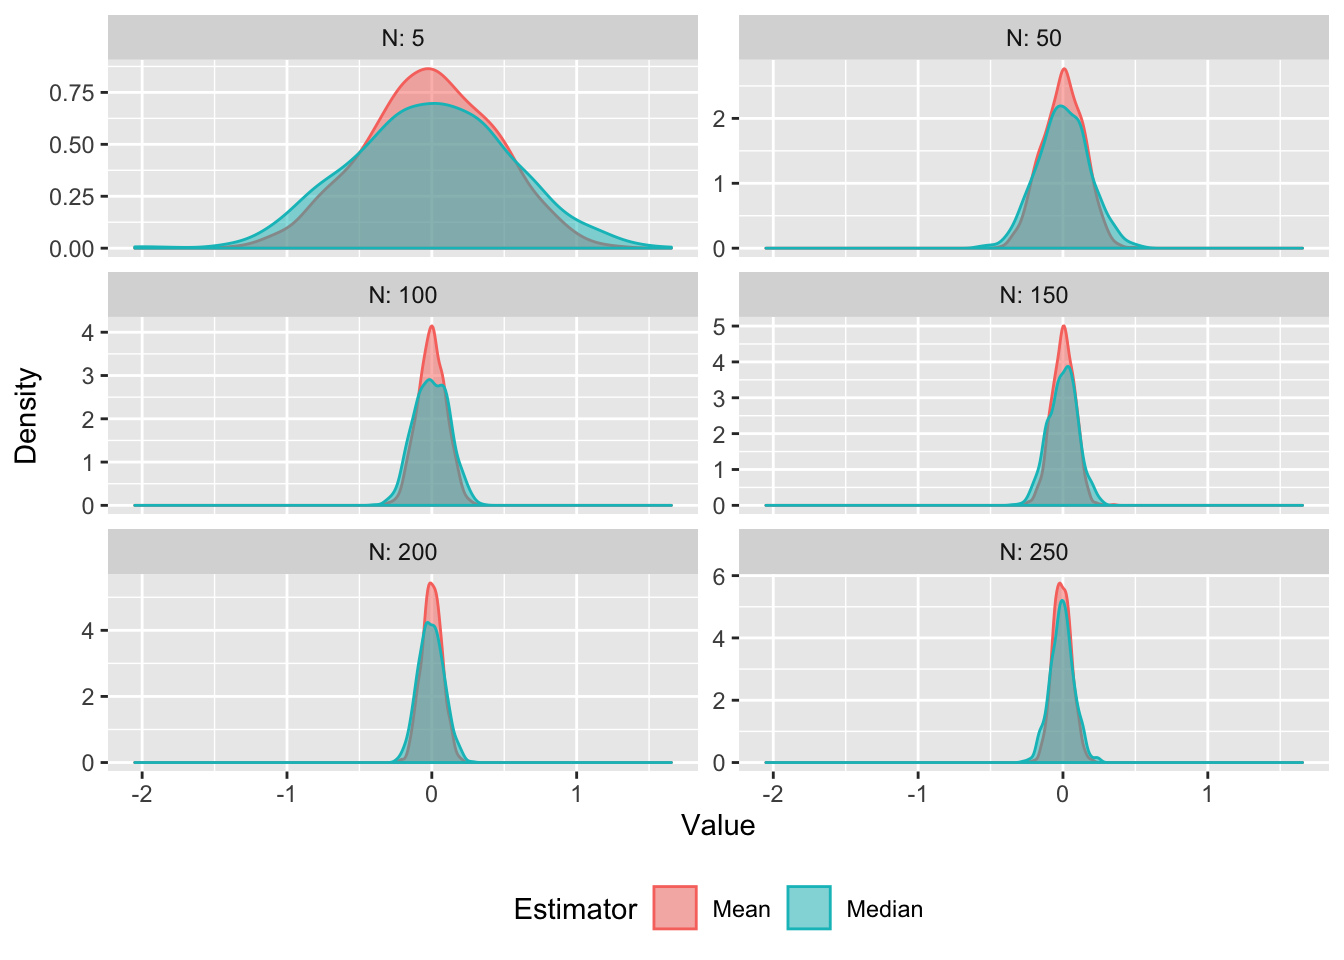
\includegraphics{10EconometricTheorems_files/figure-latex/unnamed-chunk-4-1.pdf}

Here we can see that for both the mean and median sample estimators, the distribution of parameters is normally distributed around the true mean (\(\theta = 0\)). The variance of the sample mean distribution, however, shrinks faster than that of the sample median estimator. In other words, the sample mean is more ``efficient'' (in fact it is the most efficient estimator). Efficiency here captures what we noted mathematically above -- that the rate of convergence on the true parameter (i.e.~the rate at which the estimator converges on zero) is faster for the sample mean than the median.

Note that both estimators are therefore unbiased (they are centred on \(\theta\)), normally distributed, and are consistent (the sampling distributions shrink towards the true parameter as N increases), but that the variances shrinks at slightly different rates.

We can quantify this using little-o notation and the behaviour of these estimators with large-samples. First, we can define the estimation errors of the mean and median respectively as

\[
\begin{aligned}
\psi_\text{Mean} &= \hat{\theta} - \theta \\ 
&= \mathcal{N}(\theta, \frac{\sigma^2}{N}) - \mathcal{N}(\theta,0) \\
&= \mathcal{N}(0,\frac{\sigma^2}{N}).
\end{aligned}
\]

Similarly,

\[
\begin{aligned}
\psi_\text{Med.} &= \mathcal{N}(\theta, \frac{\pi\sigma^2}{2N}) - \mathcal{N}(\theta,0)  \\
& = \mathcal{N}(0, \frac{\pi\sigma^2}{2N}).
\end{aligned}
\]

With both mean and median expressions, we can see that the error of the estimators is centered around zero (i.e.~it is unbiased), and that the dispersion of the error around zero decreases as \(N\) increases. Given earlier discussions in this chapter, we can rearrange both to find out their rate of convergence.

For the sample mean:

\[ 
\begin{aligned}
\psi_\text{Mean} &= \frac{1}{\sqrt{N}}\mathcal{N}(0,\sigma^2) \\
\frac{\psi_\text{Mean}}{N^{-0.5}} &= \mathcal{N}(0,\sigma^2)
\end{aligned}
\]

We know that for a normal distribution, there will be some \(M_\epsilon\), \(N_\epsilon\), such that \(P(|\mathcal{N}(0,\sigma^2)| \geq M_\epsilon) < \epsilon\), and hence:

\[\psi_\text{Mean} = O_p(\frac{1}{\sqrt{N}}).\]
Similarly, for the sample median:

\[ 
\begin{aligned}
\psi_\text{Med.} &= \mathcal{N}(0, \frac{\pi\sigma^2}{2N}) \\
&= \left( \frac{\pi}{2N}\right)^{0.5}\mathcal{N}(0,\sigma^2) \\
\psi_\text{Med.}/\left( \frac{\pi}{2N}\right)^{0.5} &= \mathcal{N}(0,\sigma^2)\\
\psi_\text{Med.} &= O_p\left( \left[\frac{\pi}{2N}\right]^{0.5}\right) \\
&= O_p\left(\frac{\sqrt{\pi}}{\sqrt{2N}}\right).
\end{aligned}
\]

Now we can see that the big-op of the sample median's estimating error is ``slower'' (read: larger) than the big-op of the sample mean, meaning that the sample mean converges on the true parameter with fewer observations than the sample median.

Another, easy way to see the intuition behind this point is to note that at intermediary steps in the above rearrangements:

\[
\begin{aligned}
\psi_\text{Mean} &= \frac{1}{\sqrt{N}}\mathcal{N}(0,\sigma^2) \\
\psi_\text{Med.} &= \frac{\sqrt{\pi}}{\sqrt{2N}}\mathcal{N}(0,\sigma^2), \\
\end{aligned}
\]
and so, for any sized sample, the estimating error of the median is larger than that of the mean. To visualise this, we can plot the estimation error as a function of \(N\) using the rates derived above:

\begin{Shaded}
\begin{Highlighting}[]
\NormalTok{N <-}\StringTok{ }\KeywordTok{seq}\NormalTok{(}\FloatTok{0.01}\NormalTok{,}\DecValTok{100}\NormalTok{, }\DataTypeTok{by =} \FloatTok{0.01}\NormalTok{)}
\NormalTok{mean_convergence <-}\StringTok{ }\DecValTok{1}\OperatorTok{/}\KeywordTok{sqrt}\NormalTok{(N)}
\NormalTok{median_convergence <-}\StringTok{ }\KeywordTok{sqrt}\NormalTok{(pi)}\OperatorTok{/}\KeywordTok{sqrt}\NormalTok{(}\DecValTok{2}\OperatorTok{*}\NormalTok{N)}

\NormalTok{plot_df <-}\StringTok{ }\KeywordTok{data.frame}\NormalTok{(N, }\DataTypeTok{Mean =}\NormalTok{ mean_convergence, }\DataTypeTok{Median =}\NormalTok{ median_convergence) }\OperatorTok\StringTok{ }
\StringTok{  }\KeywordTok{pivot_longer}\NormalTok{(}\OperatorTok{-}\NormalTok{N, }\DataTypeTok{names_to =} \StringTok{"Estimator"}\NormalTok{, }\DataTypeTok{values_to =} \StringTok{"Rate"}\NormalTok{)}

\KeywordTok{ggplot}\NormalTok{(plot_df, }\KeywordTok{aes}\NormalTok{(}\DataTypeTok{x =}\NormalTok{ N, }\DataTypeTok{y =}\NormalTok{ Rate, }\DataTypeTok{color =}\NormalTok{ Estimator)) }\OperatorTok{+}
\StringTok{  }\KeywordTok{geom_line}\NormalTok{() }\OperatorTok{+}
\StringTok{  }\KeywordTok{ylim}\NormalTok{(}\DecValTok{0}\NormalTok{,}\DecValTok{1}\NormalTok{) }\OperatorTok{+}
\StringTok{  }\KeywordTok{theme}\NormalTok{(}\DataTypeTok{legend.position =} \StringTok{"bottom"}\NormalTok{)}
\end{Highlighting}
\end{Shaded}

\begin{figure}
\centering
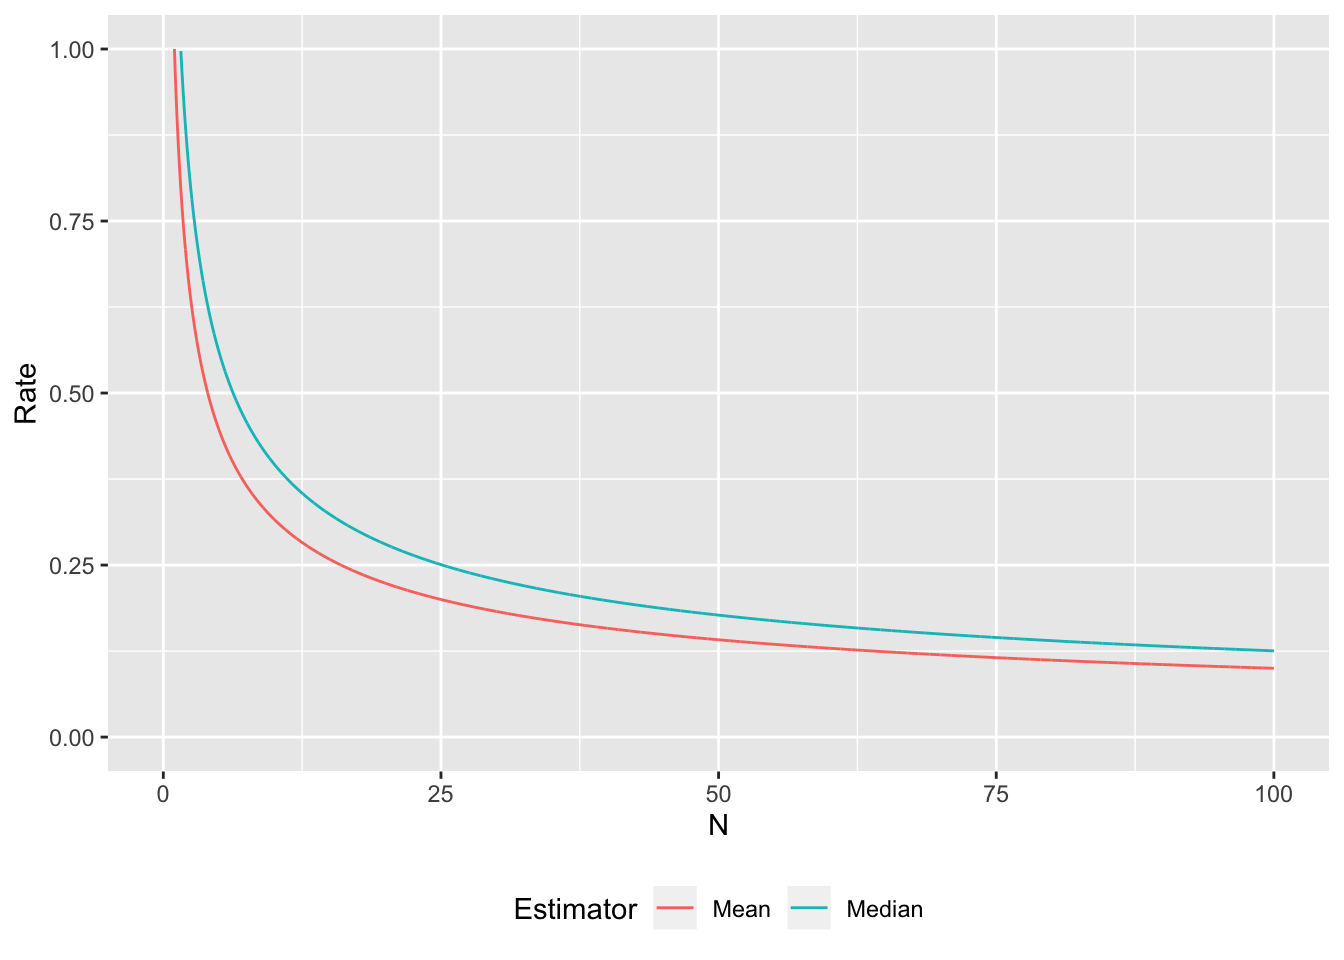
\includegraphics{10EconometricTheorems_files/figure-latex/unnamed-chunk-5-1.pdf}
\caption{\label{fig:unnamed-chunk-5}Simulated distribution of sample mean and median estimators for different sized samples.}
\end{figure}

Note that the median rate line is always above the mean line for all \(N\) (though not by much) -- it therefore has a slower convergence.

\hypertarget{dm}{%
\chapter{Delta Method}\label{dm}}

\hypertarget{delta-method-in-plain-english}{%
\section{Delta Method in Plain English}\label{delta-method-in-plain-english}}

The Delta Method (DM) states that we can approximate the asymptotic behaviour of functions over a random variable, if the random variable is itself asymptotically normal. In practice, this theorem tells us that even if we do not know the expected value and variance of the function \(g(X)\) we can still approximate it reasonably. Note that by \protect\hyperlink{clt}{Central Limit Theorem} we know that several important random variables and estimators are asymptotically normal, including the sample mean. We can therefore approximate the mean and variance of some transformation of the sample mean using its variance.

More specifically, suppose that we have some sequence of random variables \(X_n\), such that as \(n\to\infty\)

\[
X_n \sim N(\mu,\frac{\sigma^2}{n}).
\]

We can rearrange this statement, to capture that the difference between the random variable and some constant \(\mu\) converges to a normal distribution around zero, with a variance determined by the number of observations:\footnote{There are clear parallels here to how we expressed \href{\%7B\#estimator_consistency\%7D\%20in\%20the\%20previous\%20chapter}{estimator consistency}.}

\[
(X_n - \mu) \sim N(0, \frac{\sigma^2}{n}).
\]

Further rearrangement yields

\[
\begin{aligned}
(X_n - \mu) &\sim \frac{\sigma}{\sqrt{n}}N(0,1) \\
\frac{\sqrt{n}(X_n - \mu)}{\sigma} &\sim N(0,1),
\end{aligned}
\]
by first moving the finite variance and \(n\) terms outside of the normal distribution, and then dividing through.

Given this, if \(g\) is some smooth function (i.e.~there are no discontinuous jumps in values) then the Delta Method states that:

\[
\frac{\sqrt{n}(g(X_n) - g(\mu))}{|g'(\mu)|\sigma} \approx N(0,1),
\]

where \(g'\) is the first derivative of \(g\). Rearranging again, we can see that

\[
g(X_n) \approx N\left(g(\mu), \frac{g'(\mu)^2\sigma^2}{n}\right).
\]

Note that the statement above is an approximation because \(g(X_n) = g(\mu) + g'(\mu)(\hat{\mu-\mu} + g''(\mu)\frac{(X_n - \mu)^2}{2!}+...\), i.e.~an infinite sum. The Delta Method avoids the infinite regress by ignoring higher order terms \citep{liu_2012}. I return to this point below in the proof.

DM also generalizes to multidimensional functions, where instead of converging on the standard normal the random variable must converge in distribution to a multivariate normal, and the derivatives of \(g\) are replaced with the gradient of g (a vector of all partial derivatives).{[}\^{}fn\_gradient{]} For the sake of simplicity I do not prove this result here, and instead focus on the univariate case.

\[ 
   \begin{aligned}
    \nabla g &= \begin{bmatrix}
           \frac{dg}{dx_1} \\
           \frac{dg}{dx_2} \\
           \vdots \\
           \frac{dg}{dx_n}
         \end{bmatrix}
  \end{aligned}
   \]

\hypertarget{proof_dm}{%
\section{Proof}\label{proof_dm}}

Before offering a full proof, we need to know a little bit about Taylor Series and Taylor's Theorem. I briefly outline this concept here, then show how this expansion helps to prove DM.

\hypertarget{taylors-series-and-theorem}{%
\subsection{Taylor's Series and Theorem}\label{taylors-series-and-theorem}}

Suppose we have some continuous function \(g\) that is infinitely differentiable. By that, we mean that we mean some function that is continuous over a domain, and for which there is always some further derivative of the function. Consider the case \(g(x) = e^{2x}\),

\[
\begin{aligned}
g'(x) &= 2e^{2x} \\
g''(x) &= 4e^{2x} \\
g'''(x) &= 8e^{2x} \\
g''''(x) &= 16e^{2x} \\
...
\end{aligned}
\]
For any integer \(k\), the \(k\)th derivative of \(g(x)\) is defined. An interesting non-infinitely differentiable function would be \(g(x) = |x|\) where \(-\infty < x < \infty\). Here note that when \(x > 0\), the first order derivative is 1 (the function is equivalent to \(x\)), and similarly at \(x <0\), the first order derivative is -1 (the function is equivalent to \(-x\)). When \(x = 0\), however, the first derivative is undefined -- the first derivative jumps discontinuously.

The Taylor Series for an infinitely differentiable function at a given point \(x=p\) is an expansion of that function in terms of an infinite sum:

\[
g(x) = g(p) + g'(p)(x-p) + \frac{g''(p)}{2!}(x-p)^2 + \frac{g'''(p)}{3!}(x-p)^3 + ...
\]

Taylor Series are useful because they allow us to approximate a function at a lower polynomial order, using Taylor's Theorem. This Theorem loosely states that, for a given point \(x=p\), we can approximate a continuous and k-times differentiable function to the \(j\)th order using the Taylor Series up to the \(j\)th derivative. In other words, if we have some continuous differentiable function \(g(x)\), its first-order approximation (i.e.~its linear approximation) at point \(p\) is defined as

\[g(p) + g'(p)(x-p).\]

To make this more concrete, consider the function \(g(x) = e^x\). The Taylor Series expansion of \(g\) at point \(x=0\) is

\[g(x) = g(0) + g'(0)(x-0) +  \frac{g''(0)}{2!}(x-0)^2 + \frac{g'''(0)}{3!}(x-0)^3 + ...\]

So up to the first order, Taylors Theorem states that

\(g(x) \approx g(0)+g'(0)(x-0) = 1 + x,\)

which is the line tangent to \(e^x\) at \(x=0\). If we consider up to the second order (the quadratic approximation) our fit would be better, and even more so if we included the third, fourth, fifth orders and so on, up until the \(\infty\)th order -- at which point the Taylor Approximation is the function precisely.

\hypertarget{proof-of-delta-method}{%
\subsection{Proof of Delta Method}\label{proof-of-delta-method}}

Given Taylor's Theorem, we know that so long as \(g\) is a continuous and derivable up to the \(k\)th derivative, where \(k \geq 2\), then at the point \(\mu\):

\[ g(X_n) \approx g(\mu) + g'(\mu)(X_n-\mu). \]

Subtracting \(g(\mu)\) we have:

\[
\left(g(X_n) - g(\mu)\right) \approx g'(\mu)(X_n-\mu).
\]
We know by CLT and our assumptions regarding \(X_n\) that \((X_n-\mu) \xrightarrow{d} N(0,\frac{\sigma^2}{n})\). Therefore we can rewrite the above as

\[
\left(g(X_n) - g(\mu)\right) \approx g'(\mu)N(0,\frac{\sigma^2}{n}),
\]

Hence, by the properties of normal distributions (multiplying by a constant, adding a constant):

\[
g(X_n) \approx N\left(g(\mu),\frac{g'(\mu)^2\sigma^2}{n}\right) \;\;\; \square
\]

\hypertarget{applied-example}{%
\section{Applied example}\label{applied-example}}

\citet{bowleretal_2006} use the DM to provide confidence intervals for predicted probabilities generated from a logistic regression. Their study involves surveying politicians' attitudes toward electoral rule changes. They estimate a logistic model of the support for change on various features of the politicians including whether they won under existing electoral rules or not. To understand how winning under existing rules affects attitudes, they then generate the predicted probabilities for losers and winners separately.

Generating predicted probabilities from a linear regression involves a non-linear transformation of an asymptotically normal parameter (the logistic coefficient), and therefore we must take account of this transformation when variance of the predicted probability.

To generate the predicted probability we use the equation

\[
\hat{p} = \frac{e^{(\hat{\alpha} + \hat{\beta}_1X_1 +...+\beta_nX_n)}}{1+e^{(\hat{\alpha} + \hat{\beta}_1X_1 + ...+\hat{\beta}_nX_n)}},
\]

where \(\hat{p}\) is the predicted probability. Estimating the variance around the predicted probability is therefore quite difficult -- it involves multiple estimators, and non-linear transformations. But we do know that, assuming i.i.d and correct functional form, the estimating error of the logistic equation is asymptotically multivariate normal on the origin. And so the authors can use DM to calculate 95 percent confidence intervals. In general, the delta method is a useful way of estimating standard and errors and confidence intervals when using (but not limited to) logistic regression and other models involving non-linear transformations of model parameters.

\hypertarget{alternative-strategies}{%
\section{Alternative strategies}\label{alternative-strategies}}

The appeal of the delta method is that it gives an analytic approximation of a function's distribution, using the asymptotic properties of some more (model) parameter. But there are alternative methods to approximating these distributions (and thus standard errors) that do not rely on deriving the order conditions of that function.

One obvious alternative is the bootstrap. For a given transformation of a random variable, calculate the output of the function \(B\) times using samples of the same size as the original sample, but with replacement and take either the standard deviation or the \(a\) and \(1-a\) percentiles of the resultant parameter distribution. This method does not require the user to calculate the derivative of a function. It is a non-parametric alternative that simply approximates the distribution itself, rather than approximates the parameters of a parametric distribution.

The bootstrap is computationally more intensive (requiring \(B\) separate samples and calculations etc.) but, on the other hand, is less technical to calculate. Moreover, the Delta Method's approximation is limited analytically by the number of terms considered in the Taylor Series expansion. While the first order Taylor Theorem may be reasonable, it may be imprecise. To improve the precision one has to undertake to find the second, third, fourth etc. order terms (which may be analytically difficult). With bootstrapping, however, you can improve precision simply by taking more samples (increasing \(B\)) \citep{KinTomWit00}.

Given the ease with which we can acquire and deploy computational resources now, perhaps the delta method is no longer as useful in applied research. But the proof and asymptotic implications remain statistically interesting and worth knowing.

\hypertarget{frisch}{%
\chapter{Frisch-Waugh-Lovell Theorem}\label{frisch}}

\hypertarget{theorem-in-plain-english}{%
\section{Theorem in plain English}\label{theorem-in-plain-english}}

The Frisch-Waugh-Lovell Theorem (FWL; after the initial proof by \citet{frisch1933partial}, and later generalisation by \citet{lovell1963seasonal}) states that:

Any predictor's regression coefficient in a multivariate model is equivalent to the regression coefficient estimated from a bivariate model in which the residualised outcome is regressed on the residualised component of the predictor; where the residuals are taken from models regressing the outcome \emph{and} the predictor on all other predictors in the multivariate regression (separately).

More formally, assume we have a multivariate regression model with \(k\) predictors:

\begin{equation}
\hat{y} = \hat{\beta}_{1}x_{1} + ... \hat{\beta}_{k}x_{k} + \epsilon. \label{eq:multi}
\end{equation}

FWL states that every \(\hat{\beta}_{j}\) in Equation \ref{eq:multi} is equal to \(\hat{\beta}^{*}_{j}\), \textit{and} the residual \(\epsilon = \epsilon^{*}\) in:

\begin{equation}
     \epsilon^{y} = \hat{\beta}^{*}_{j}\epsilon^{x_j} + \epsilon^{*} 
\end{equation}

where:

\begin{align}
\begin{aligned}
     \epsilon^y & = y - \sum_{k \neq j}\hat{\beta}^{y}_{k}x_{k} \\
     \epsilon^{x_{j}} &= x_j - \sum_{k \neq j}\hat{\beta}^{x_{j}}_{k}x_{k}.
\end{aligned}
\end{align}

where \(\hat{\beta}^{y}_k\) and \(\hat{\beta}^{x_j}_k\) are the regression coefficients from two separate regression models of the outcome (omitting \(x_j\)) and \(x_j\) respectively.

In other words, FWL states that each predictor's coefficient in a multivariate regression explains that variance of \(y\) not explained by both the other k-1 predictors' relationship with the outcome and their relationship with that predictor, i.e.~the independent effect of \(x_j\).

\hypertarget{proof_fw}{%
\section{Proof}\label{proof_fw}}

\hypertarget{primer-projection-matricessecnote}{%
\subsection[Primer: Projection matrices]{\texorpdfstring{Primer: Projection matrices\footnote{\emph{Citation} Based on \href{https://www.uio.no/studier/emner/sv/oekonomi/ECON4160/h13/undervisningsmateriale/lnote1h13-.pdf}{lecture notes} from the University of Oslo's ``Econometrics -- Modelling and Systems Estimation" course (author attribution unclear), and \citet{davidson2004econometric}.\}}}{Primer: Projection matrices}}\label{primer-projection-matricessecnote}}

We need two important types of projection matrices to understand the linear algebra proof of FWL. First, the \textbf{prediction matrix} that was introduced in \protect\hyperlink{linear_projection}{Chapter 4}:

\begin{equation}
    P = X(X'X)^{-1}X'.
\end{equation}

Recall that this matrix, when applied to an outcome vector (\(y\)), produces a set of predicted values (\(\hat{y}\)). Reverse engineering this, note that \(\hat{y}=X\hat{\beta}=X(X'X)^{-1}X'y = Py\).

Since \(Py\) produces the predicted values from a regression on \(X\), we can define its complement, the \textbf{residual maker}:

\begin{equation}
    M = I - X(X'X)^{-1}X',
\end{equation}

since \(My = y - X(X'X)^{-1}X'y \equiv y-Py \equiv y - X\hat{\beta} \equiv \hat{\epsilon},\) the residuals from regressing \(Y\) on \(X\).

Given these definitions, note that M and P are complementary:

\begin{align}
\begin{aligned}
    y  &= \hat{y} + \hat{\epsilon} \\
       &\equiv Py + My \\ 
    Iy &= Py + My \\
    Iy &= (P + M)y \\
    I  &= P + M.
\end{aligned}
\end{align}

With these projection matrices, we can express the FWL claim (which we need to prove) as:

\begin{align}
\begin{aligned}
    y &= X_{1}\hat{\beta_{1}} + X_{2}\hat{\beta_{2}} + \hat{\epsilon} \\
    M_{1}y &= M_{1}X_2\hat{\beta}_{2} + \hat{\epsilon}, \label{projection_statement}
\end{aligned}
\end{align}

\hypertarget{fwl-proof-secnote2}{%
\subsection[FWL Proof ]{\texorpdfstring{FWL Proof \footnote{\emph{Citation}: Adapted from York University, Canada's \href{http://scs.math.yorku.ca/index.php/Statistics:_Frisch-Waugh-Lovell_and_GLS/Proof_of_the_FWL_for_OLS}{wiki for statistical consulting}.}}{FWL Proof }}\label{fwl-proof-secnote2}}

Let us assume, as in Equation \ref{projection_statement} that:

\begin{equation}
    Y = X_1\hat{\beta}_1 + X_2\hat{\beta}_2 + \hat{\epsilon}. \label{eq:multivar}
\end{equation}

First, we can multiply both sides by the residual maker of \(X_1\):

\begin{equation}
    M_1Y = M_1X_1\hat{\beta}_1 + M_1X_2\hat{\beta}_2 + M_1\hat{\epsilon},
\end{equation}

which first simplifies to:

\begin{equation}
    M_1Y = M_1X_2\hat{\beta}_2 + M_1\hat{\epsilon}, \label{eq:part_simp}
\end{equation}

because \(M_1X_1\hat{\beta}_1 \equiv (M_1X_1)\hat{\beta}_1 \equiv 0\hat{\beta}_1 = 0\). In plain English, by definition, all the variance in \(X_1\) is explained by \(X_1\) and therefore a regression of \(X_1\) on itself leaves no part unexplained so \(M_1X_1\) is zero.\footnote{Algebraically, $M_1X_1 = (I-X_1(X_{1}'X_1)^{-1}X_1')X_1 = X_1 - X_1(X_1'X_1)^{-1}X_1'X = X_1 - X_1I = X_1 - X_1 = 0.$}

Second, we can simplify this equation further because, by the properties of OLS regression, \(X_1\) and \(\epsilon\) are orthogonal. Therefore the residual of the residuals are the residuals! Hence:

\begin{equation*}
    M_1Y = M_1X_2\hat{\beta}_2 + \hat{\epsilon} \; \; \; \square.
\end{equation*}

\subsection{Interesting features/extensions}

A couple of interesting features come out of the linear algebra proof:

\begin{itemize}
\item
  FWL also holds for bivariate regression when you first residualise Y and X on a \(n\times1\) vector of 1's (i.e.~the constant) -- which is like demeaning the outcome and predictor before regressing the two.
\item
  \(X_1\) and \(X_2\) are technically \textit{sets} of mutually exclusive predictors i.e.~\(X_1\) is an \(n \times k\) matrix \(\{X_1,...,X_k\}\), and \(X_2\) is an \(n \times m\) matrix \(\{X_{k+1},...,X_{k+m}\}\), where \(\beta_1\) is a corresponding vector of regression coefficients \(\beta_1 = \{\gamma_1,...,\gamma_k\}\), and likewise \(\beta_2 = \{\delta_1,..., \delta_m\}\), such that:

  \begin{align*}
    Y &= X_1\beta_1 + X_2\beta_2 \\
      &= X_{1}\hat{\gamma}_1 + ... + X_{k}\hat{\gamma}_k + X_{k+1}\hat{\delta}_{1} + ... + X_{k+m}\hat{\delta}_{m},
    \end{align*}
\end{itemize}

Hence the FWL theorem is exceptionally general, applying not only to arbitrarily long coefficient vectors, but also enabling you to back out estimates from any partitioning of the full regression model.

\hypertarget{coded-example}{%
\section{Coded example}\label{coded-example}}

\begin{Shaded}
\begin{Highlighting}[]
\KeywordTok{set.seed}\NormalTok{(}\DecValTok{89}\NormalTok{)}

\CommentTok{## Generate random data}
\NormalTok{df <-}\StringTok{ }\KeywordTok{data.frame}\NormalTok{(}\DataTypeTok{y =} \KeywordTok{rnorm}\NormalTok{(}\DecValTok{1000}\NormalTok{,}\DecValTok{2}\NormalTok{,}\FloatTok{1.5}\NormalTok{),}
                 \DataTypeTok{x1 =} \KeywordTok{rnorm}\NormalTok{(}\DecValTok{1000}\NormalTok{,}\DecValTok{1}\NormalTok{,}\FloatTok{0.3}\NormalTok{),}
                 \DataTypeTok{x2 =} \KeywordTok{rnorm}\NormalTok{(}\DecValTok{1000}\NormalTok{,}\DecValTok{1}\NormalTok{,}\DecValTok{4}\NormalTok{))}

\CommentTok{## Partial regressions}

\CommentTok{# Residual of y regressed on x1}
\NormalTok{y_res <-}\StringTok{ }\KeywordTok{lm}\NormalTok{(y }\OperatorTok{~}\StringTok{ }\NormalTok{x1, df)}\OperatorTok{$}\NormalTok{residuals}

\CommentTok{# Residual of x2 regressed on x1}
\NormalTok{x_res <-}\StringTok{ }\KeywordTok{lm}\NormalTok{(x2 }\OperatorTok{~}\StringTok{ }\NormalTok{x1, df)}\OperatorTok{$}\NormalTok{residuals}

\NormalTok{resids <-}\StringTok{ }\KeywordTok{data.frame}\NormalTok{(y_res, x_res)}

\CommentTok{## Compare the beta values for x2}
\CommentTok{# Multivariate regression:}
\KeywordTok{summary}\NormalTok{(}\KeywordTok{lm}\NormalTok{(y}\OperatorTok{~}\NormalTok{x1}\OperatorTok{+}\NormalTok{x2, df))}
\end{Highlighting}
\end{Shaded}

\begin{verbatim}
## 
## Call:
## lm(formula = y ~ x1 + x2, data = df)
## 
## Residuals:
##    Min     1Q Median     3Q    Max 
## -4.451 -1.001 -0.039  1.072  5.320 
## 
## Coefficients:
##             Estimate Std. Error t value Pr(>|t|)    
## (Intercept)  2.33629    0.16427  14.222   <2e-16 ***
## x1          -0.31093    0.15933  -1.952   0.0513 .  
## x2           0.02023    0.01270   1.593   0.1116    
## ---
## Signif. codes:  0 '***' 0.001 '**' 0.01 '*' 0.05 '.' 0.1 ' ' 1
## 
## Residual standard error: 1.535 on 997 degrees of freedom
## Multiple R-squared:  0.006252,	Adjusted R-squared:  0.004258 
## F-statistic: 3.136 on 2 and 997 DF,  p-value: 0.04388
\end{verbatim}

\begin{Shaded}
\begin{Highlighting}[]
\CommentTok{# Partials regression}
\KeywordTok{summary}\NormalTok{(}\KeywordTok{lm}\NormalTok{(y_res }\OperatorTok{~}\StringTok{ }\NormalTok{x_res, resids))}
\end{Highlighting}
\end{Shaded}

\begin{verbatim}
## 
## Call:
## lm(formula = y_res ~ x_res, data = resids)
## 
## Residuals:
##    Min     1Q Median     3Q    Max 
## -4.451 -1.001 -0.039  1.072  5.320 
## 
## Coefficients:
##               Estimate Std. Error t value Pr(>|t|)
## (Intercept) -8.921e-17  4.850e-02   0.000    1.000
## x_res        2.023e-02  1.270e-02   1.593    0.111
## 
## Residual standard error: 1.534 on 998 degrees of freedom
## Multiple R-squared:  0.002538,	Adjusted R-squared:  0.001538 
## F-statistic: 2.539 on 1 and 998 DF,  p-value: 0.1114
\end{verbatim}

\textbf{Note:} This isn't an exact demonstration because there is a degrees of freedom of error. The (correct) multivariate regression degrees of freedom is calculated as \(N - 3\) since there are three variables. In the partial regression the degrees of freedom is \(N - 2\). This latter calculation does not take into account the additional loss of freedom as a result of partialling out \(X_1\).

\hypertarget{application-sensitivity-analysis}{%
\section{Application: Sensitivity analysis}\label{application-sensitivity-analysis}}

\citet{cinelli2020making} develop a series of tools for researchers to conduct sensitivity analyses on regression models, using an extension of the omitted variable bias framework. To do so, they use FWL to motivate this bias. Suppose that the full regression model is specified as:

\begin{equation}
    Y = \hat{\tau}D + X\hat{\beta} + \hat{\gamma}Z + \hat{\epsilon}_{\text{full}}, \label{eq:ch_full}
\end{equation}

where \(\hat{\tau}, \hat{\beta}, \hat{\gamma}\) are estimated regression coefficients, D is the treatment variable, X are observed covariates, and Z are unobserved covariates. Since, Z is unobserved, researchers measure:

\begin{equation}
Y = \hat{\tau}_\text{Obs.}D + X\hat{\beta}_\text{Obs.} + \epsilon_\text{Obs}
\end{equation}

By FWL, we know that \(\hat{\tau}_\text{Obs.}\) is equivalent to the coefficient of regressing the residualised outcome (with respect to X), on the residualised outcome of D (again with respect to X). Call these two residuals \(Y_r\) and \(D_r\).

And recall that the regression model for the final-stage of the partial regressions is bivariate (\(Y_r \sim D_r\)). Conveniently, a bivariate regression coefficient can be expressed in terms of the covariance between the left-hand and right-hand side variables:\footnote{If $y = \hat{\alpha} + \hat{\beta}x + \epsilon$, then by least squares $\hat{\beta} = \frac{cov(x,y)}{var(x)}$ and $\hat{\alpha} = \bar{y} - \hat{\beta}\bar{x}$.}

\begin{equation}
    \hat{\tau}_\text{Obs.} = \frac{cov(D_r, Y_r)}{var(D_r)}.
\end{equation}

Note that given the full regression model in Equation \ref{eq:ch_full}, the partial outcome \(Y_r\) is actually composed of the elements \(\hat{\tau}D_r + \hat{\gamma}Z_r\), and so:

\begin{equation}
    \hat{\tau}_\text{Obs.} = \frac{cov(D_r, \hat{\tau}D_r + \hat{\gamma}Z_r)}{var(D_r)} \label{eq:cov_expand}
\end{equation}

Next, we can expand the covariance using the expectation rule that \(cov(A, B+C) = cov(A,B) + cov(A,C)\) and since \(\hat{\tau},\hat{\gamma}\) are scalar, we can move them outside the covariance functions:

\begin{equation}
    \hat{\tau}_\text{Obs.} = \frac{\hat{\tau}cov(D_r, D_r) + \hat{\gamma}cov(D_r,Z_r)}{var(D_r)}
\end{equation}

Since \(cov(A,A) = var(A)\) and therefore:

\begin{equation}
    \hat{\tau}_\text{Obs.} = \frac{\hat{\tau}var(D_r) + \hat{\gamma}cov(D_r,Z_r)}{var(D_r)} \equiv \hat{\tau} + \hat{\gamma}\frac{cov(D_r,Z_r)}{var(D_r)} \equiv \hat{\tau} + \hat{\gamma}\hat{\delta}
\end{equation}

Frisch-Waugh is so useful because it simplifies a multivariate equation into a bivariate one. While computationally this makes zero difference (unlike in the days of hand computation), here it allows us to use a convenient expression of the bivariate coefficient to show and quantify the bias when you run a regression in the presence of an unobserved confounder. Moreover, note that in Equation \ref{eq:cov_expand}, we implicitly use FWL again since we know that the non-stochastic aspect of Y not explained by X are the residualised components of the full Equation \ref{eq:ch_full}.

\hypertarget{regressing-the-partialled-out-x-on-the-full-y}{%
\subsection{Regressing the partialled-out X on the full Y}\label{regressing-the-partialled-out-x-on-the-full-y}}

In \emph{Mostly Harmless Econometrics} (MHE; \citet{AngristMostlyHarmlessEconometrics2009}), the authors note that you also get an identical coefficient to the full regression if you regress the residualised predictor on the non-residualised \(Y\). We can use the OVB framework above to explain this case.

Let's take the full regression model as:

\begin{equation}
Y = \hat{\beta}_1X_1 + \hat{\beta}_2X_2 + \hat{\epsilon}.    
\end{equation}

\textit{MHE} states that:

\begin{equation}
    Y = \hat{\beta_1}M_2X_1 + \hat{\epsilon}.
\end{equation}

Note that this is just FWL, except we have not also residualised \(Y\). Our aim is to check whether there is any bias in the estimated coefficient from this second equation. As before, since this is a bivariate regression we can express the coefficient as:

\begin{align}
    \begin{aligned}
    \hat{\beta}_1 &= \frac{cov(M_2X_1, Y)}{var(M_2X_1)} \\
    &= \frac{cov(M_2X_1, \hat{\beta}_1X_1 + \hat{\beta}_2X_2)}{var(M_2X_1)} \\
    &= \hat{\beta}_1\frac{cov(M_2X_1,X_1)}{var(M_2X_1)} + \hat{\beta}_2\frac{cov(M_2X_1,X_2)}{var(M_2X_1)} \\
    &= \hat{\beta}_1 + \hat{\beta}_2\times 0 \\
    &= \hat{\beta}_1
    \end{aligned}
\end{align}

This follows from two features. First, \(cov(M_2X_1,X_1) = var(M_2X_1)\). Second, it is clear that \(cov(M_2X_1, X_2) =0\) because \(M_2X_1\) is \(X_1\) stripped of any variance associated with \(X_2\) and so, by definition, they do not covary. Therefore, we can recover the unbiased regression coefficient using an adapted version of FWL where we do not residualise Y -- as stated in \emph{MHE}.

\hypertarget{pd}{%
\chapter{Positive Definite Matrices}\label{pd}}

\hypertarget{pd_terms}{%
\section{Terminology}\label{pd_terms}}

A \(n \times n\) symmetric matrix \(M\) is \emph{positive definite (PD)} if and only if \(x'Mx > 0\), for all \emph{non-zero} \(x \in \mathbb{R}^n\). For example, take the \(3 \times 3\) identity matrix, and a column vector of non-zero real numbers \([a,b,c]\):

\[
\begin{aligned}
\begin{bmatrix}
a & b & c
\end{bmatrix}
\begin{bmatrix}
1 & 0 & 0\\
0 & 1 & 0 \\
0 & 0 & 1
\end{bmatrix}
\begin{bmatrix}
a \\
b \\
c
\end{bmatrix} \\
= \begin{bmatrix}
a & b & c
\end{bmatrix}
\begin{bmatrix}
a \\
b \\
c
\end{bmatrix} \\
= a^2 + b^2 + c^2.
\end{aligned}
\]

Since by definition \(a^2, b^2,\) and \(c^2\) are all greater than zero (even if \(a,b,\) or \(c\) are negative), their sum is also positive.

A matrix is \emph{positive semi-definite (PSD)} if and only if \(x'Mx \geq 0\) for all non-zero \(x \in \mathbb{R}^n\). Note that PSD differs from PD in that the transformation of the matrix is no longer \emph{strictly} positive.

One known feature of matrices (that will be useful later in this chapter) is that if a matrix is symmetric and idempotent then it will be positive semi-definite. Take some non-zero vector \(x\), and a symmetric, idempotent matrix \(A\). By idempotency we know that \(x'Ax = x'AAx\). By symmetry we know that \(A' = A\), and therefore:

\[
\begin{aligned}
x'Ax &= x'AAx \\
&= x'A'Ax \\
&= (Ax)'Ax \geq 0,
\end{aligned}
\]

and hence PSD.\footnote{This short proof is taken from \href{https://www.reddit.com/r/math/comments/9ni2x/why_does_symmetry_and_idempotence_imply}{this discussion}.}

\hypertarget{positivity}{%
\subsection{Positivity}\label{positivity}}

Both PD and PSD are concerned with positivity. For scalar values like -2, 5, 89, positivity simply refers to their sign -- and we can tell immediately whether the numbers are positive or not. Some functions are also (strictly) positive. Think about \(f(x) = x^2 + 1\). For all \(x \in \mathbb{R}\), \(f(x) \geq 1 > 0\). PD and PSD extend this notion of a positivity to matrices, which is useful when we consider multidimensional optimisation problems or the combination of matrices.

While for abstract matrices like the identity matrix it is easy to verify PD and PSD properties, for more complicated matrices we often require other more complicated methods. For example, we know that a symmetric matrix is PSD if and only if all its \emph{eigenvalues} are non-negative. The eigenvalue \(\lambda\) is a scalar such that, for a matrix \(A\) and non-zero \(n\times 1\) vector \(v\), \(A\cdot v = \lambda \cdot v\). While I do not explore this further in this chapter, there are \href{https://lpsa.swarthmore.edu/MtrxVibe/EigMat/MatrixEigen.html}{methods available} for recovering these values from the preceding equation. Further discussion of the full properties of PD and PSD matrices can be found \href{http://theanalysisofdata.com/probability/C_4.html}{here} as well as in print \citep[e.g.~][Chapter 7]{horn_2013}.

\hypertarget{a-b-is-psd-iff-b-1---a-1-is-psd}{%
\section{\texorpdfstring{\(A-B\) is PSD iff \(B^{-1} - A^{-1}\) is PSD}{A-B is PSD iff B\^{}\{-1\} - A\^{}\{-1\} is PSD}}\label{a-b-is-psd-iff-b-1---a-1-is-psd}}

Wooldridge's list of 10 theorems does not actually include a general claim about the importance P(S)D matrices. Instead, he lists a very specific feature of two PD matrices. In plain English, this theorem states that, assuming \(A\) and \(B\) are both positive definite, \(A-B\) is positive semi-definite if and only if the inverse of \(B\) minus the inverse of \(A\) is positive semi-definite.

Before we prove this theorem, it's worth noting a few points that are immediately intuitive from its statement. Note that the theorem moves from PD matrices to PSD matrices. This is because we are subtracting one matrix from another. While we know A and B are both PD, if they are both equal then \(x'(A-B)x\) will equal zero. For example, if \(A = B = I_2 = \big(\begin{smallmatrix} 1 & 0\\ 0 & 1 \end{smallmatrix}\big)\), then \(A-B = \big(\begin{smallmatrix} 0 & 0\\ 0 & 0 \end{smallmatrix}\big)\). Hence, \(x'(A-B)x = 0\) and therefore \(A-B\) is PSD, but not PD.

Also note that this theorem only applies to a certain class of matrices, namely those we know to be PD. This hints at the sort of applied relevance this theorem may have. For instance, we know that variance is a strictly positive quantity.

The actual applied relevance of this theorem is not particularly obvious, at least from the claim alone. In his post, Wooldridge notes that he repeatedly uses this fact `to show the asymptotic efficiency of various estimators.' In his \emph{Introductory Economics} textbook \citeyearpar{Wooldridge_intro}, for instance, Wooldridge makes use of the properties of PSD matrices in proving that the Gauss-Markov (GM) assumptions ensure that OLS is the best, linear, unbiased estimator (BLUE). And, more generally, PD and PSD matrices are very helpful in optimisation problems (of relevance to machine learning too). Neither appear to be direct applications of this specific, bidirectional theorem. In the remainder of this chapter, therefore, I prove the theorem itself for completeness. I then broaden the discussion to explore how PSD properties are used in Wooldridge's BLUE proof as well as discuss the more general role of PD matrices in optimisation problems.

\hypertarget{pd_proof}{%
\subsection{Proof}\label{pd_proof}}

The proof of Wooldridge's actual claim is straightforward. In fact, given the symmetry of the proof, we only need to prove one direction (i.e.~if \(A-B\) is PSD, then \(A^{-1} - B^{-1}\) is PSD.)

Let's assume, therefore, that \(A - B\) is PSD. Hence:

\[
\begin{aligned}
x'(A-B)x &\geq 0 \\
x'Ax - xBx &\geq 0 \\
x'Ax &\geq x'Bx \\
Ax &\geq Bx \\
A &\geq B.
\end{aligned}
\]

Next, we can invert our two matrices while maintaining the inequality:

\[
\begin{aligned}
A^{-1}AB^{-1} &\geq A^{-1}BB^{-1} \\
IB^{-1} &\geq A^{-1}I \\
B^{-1} &\geq A^{-1}.
\end{aligned}
\]

Finally, we can just remultiply both sides of the inequality by our arbitrary non-zero vector:

\[
\begin{aligned}
x'B^{-1} &\geq x'A^{-1} \\
x'B^{-1}x &\geq x'A^{-1}x \\
x'B^{-1}x - x'A^{-1}x &\geq 0 \\
x'(B^{-1} - A^{-1})x &\geq 0.
\end{aligned}
\]

Proving the opposite direction (if \(B^{-1} - A^{-1}\) is PSD then \(A-B\) is PSD) simply involves replacing A with \(B^{-1}\) an \(B\) with \(A^{-1}\) and \emph{vice versa} throughout the proof, since \((A^{-1})^{-1} = A. \;\;\;\square\)

\hypertarget{pd_app}{%
\section{Applications}\label{pd_app}}

\hypertarget{ols-as-the-best-linear-unbiased-estimator-blue}{%
\subsection{OLS as the best linear unbiased estimator (BLUE)}\label{ols-as-the-best-linear-unbiased-estimator-blue}}

First, let's introduce the four Gauss-Markov assumptions. I only state these briefly, in the interest of space, spending a little more time explaining the rank of a matrix. Collectively, these assumptions guarantee that the linear regression estimates \(\hat{\beta}\) are BLUE (the best linear unbiased estimator of \(\beta\)).

\begin{enumerate}
\def\labelenumi{\arabic{enumi}.}
\item
  The true model is linear such that \(y = X\beta + u\), where \(y\) is a \(n \times 1\) vector, \(X\) is a \(n \times (k + 1)\) matrix, and \(u\) is an unobserved \(n \times 1\) vector.
\item
  The rank of \(X\) is \((k+1)\) (full-rank), i.e.~that there are no linear dependencies among the variables in \(X\). To understand what the rank of matrix denotes, consider the following \(3\times 3\) matrix:
\end{enumerate}

\[
  M_1=\begin{bmatrix}
  1 & 0 & 0 \\
  0 & 1 & 0 \\
  2 & 0 & 0
  \end{bmatrix}
  \]

Note that the third row of \(M_1\) is just two times the first column. They are therefore entirely linearly dependent, and so not separable. The number of independent rows (the rank of the matrix) is therefore 2. One way to think about this geometrically, as in \protect\hypertarget{linear_projection}{}{Chapter 3}, is to plot each row as a vector. The third vector would completely overlap the first, and so in terms of direction we would not be able to discern between them. In terms of the span of these two columns, moreover, there is no point that one can get to using a combination of both that one could not get to by scaling either one of them.

A slightly more complicated rank-deficient (i.e.~not full rank) matrix would be:

\[
  M_2=\begin{bmatrix}
  1 & 0 & 0 \\
  0 & 1 & 0 \\
  2 & 1 & 0
  \end{bmatrix}
  \]

Here note that the third row is not scalar multiple of either other column. But, it is a linear combination of the other two. If rows 1, 2, and 3 are represented by \(a, b,\) and \(c\) respectively, then \(c = 2a + b\). Again, geometrically, there is no point that the third row vector can take us to which cannot be achieved using only the first two rows.

An example of a matrix with full-rank, i.e.~no linear dependencies, would be:

\[
  M_2=\begin{bmatrix}
  1 & 0 & 0 \\
  0 & 1 & 0 \\
  2 & 0 & 1
  \end{bmatrix}
  \]

It is easy to verify that \(M_1\) and \(M_2\) are rank-deficient, whereas \(M_3\) is of full-rank in R:

\begin{Shaded}
\begin{Highlighting}[]
\NormalTok{M1 <-}\StringTok{ }\KeywordTok{matrix}\NormalTok{(}\KeywordTok{c}\NormalTok{(}\DecValTok{1}\NormalTok{,}\DecValTok{0}\NormalTok{,}\DecValTok{2}\NormalTok{,}\DecValTok{0}\NormalTok{,}\DecValTok{1}\NormalTok{,}\DecValTok{0}\NormalTok{,}\DecValTok{0}\NormalTok{,}\DecValTok{0}\NormalTok{,}\DecValTok{0}\NormalTok{), }\DataTypeTok{ncol =} \DecValTok{3}\NormalTok{)}
\NormalTok{M1_rank <-}\StringTok{ }\KeywordTok{qr}\NormalTok{(M1)}\OperatorTok{$}\NormalTok{rank}

\NormalTok{M2 <-}\StringTok{ }\KeywordTok{matrix}\NormalTok{(}\KeywordTok{c}\NormalTok{(}\DecValTok{1}\NormalTok{,}\DecValTok{0}\NormalTok{,}\DecValTok{2}\NormalTok{,}\DecValTok{0}\NormalTok{,}\DecValTok{1}\NormalTok{,}\DecValTok{1}\NormalTok{,}\DecValTok{0}\NormalTok{,}\DecValTok{0}\NormalTok{,}\DecValTok{0}\NormalTok{), }\DataTypeTok{ncol =} \DecValTok{3}\NormalTok{)}
\NormalTok{M2_rank <-}\StringTok{ }\KeywordTok{qr}\NormalTok{(M2)}\OperatorTok{$}\NormalTok{rank}

\NormalTok{M3 <-}\StringTok{ }\KeywordTok{matrix}\NormalTok{(}\KeywordTok{c}\NormalTok{(}\DecValTok{1}\NormalTok{,}\DecValTok{0}\NormalTok{,}\DecValTok{2}\NormalTok{,}\DecValTok{0}\NormalTok{,}\DecValTok{1}\NormalTok{,}\DecValTok{0}\NormalTok{,}\DecValTok{0}\NormalTok{,}\DecValTok{0}\NormalTok{,}\DecValTok{1}\NormalTok{), }\DataTypeTok{ncol =} \DecValTok{3}\NormalTok{)}
\NormalTok{M3_rank <-}\KeywordTok{qr}\NormalTok{(M3)}\OperatorTok{$}\NormalTok{rank}

\KeywordTok{print}\NormalTok{(}\KeywordTok{paste}\NormalTok{(}\StringTok{"M1 rank:"}\NormalTok{, M1_rank))}
\end{Highlighting}
\end{Shaded}

\begin{verbatim}
## [1] "M1 rank: 2"
\end{verbatim}

\begin{Shaded}
\begin{Highlighting}[]
\KeywordTok{print}\NormalTok{(}\KeywordTok{paste}\NormalTok{(}\StringTok{"M2 rank:"}\NormalTok{, M2_rank))}
\end{Highlighting}
\end{Shaded}

\begin{verbatim}
## [1] "M2 rank: 2"
\end{verbatim}

\begin{Shaded}
\begin{Highlighting}[]
\KeywordTok{print}\NormalTok{(}\KeywordTok{paste}\NormalTok{(}\StringTok{"M3 rank:"}\NormalTok{, M3_rank))}
\end{Highlighting}
\end{Shaded}

\begin{verbatim}
## [1] "M3 rank: 3"
\end{verbatim}

\begin{enumerate}
\def\labelenumi{\arabic{enumi}.}
\setcounter{enumi}{2}
\item
  \(\mathbb{E}[u|X] = 0\) i.e.~that the model has zero conditional mean or, in other words, our average error is zero.
\item
  \(\text{Var}(u_i|X) = \sigma^2, \text{Cov}(u_i,u_j|X) = 0\) for all \(i \neq j\), or equivalently that \(Var(u|X) = \sigma^2I_n\). This matrix has diagonal elements all equal to \(\sigma^2\) and all off-diagonal elements equal to zero.
\end{enumerate}

BLUE states that the regression coefficient vector \(\hat{\beta}\) is the best, or lowest variance, estimator of the true \(\beta\). \citet{Wooldridge_intro} has a nice onproof of this claim (p.812). Here I unpack hisi proof in slightly more detail, noting specifically how PD matrices are used.

To begin our proof of BLUE, let us denote any other linear estimator as \(\tilde{\beta} = A'y\), where \(A\) is some \(n \times (k+1)\) matrix consisting of functions of \(X\).

We know by definition that \(y = X\beta + u\) and therefore that:

\[
\tilde{\beta} = A'(X\beta + u) = A'X\beta + A'u.
\]

The conditional expectation of \(\tilde{\beta}\) can be expressed as:

\[
\mathbb{E}(\tilde{\beta}|X) = A'X\beta + \mathbb{E}(A'u|X),
\]

and since \(A\) is a function of \(X\), we can move it outside the expectation:

\[
\mathbb{E}(\tilde{\beta}|X) = A'X\beta + A'\mathbb{E}(u|X).
\]

By the GM assumption no. 3, we know that \(\mathbb{E}(u|X) = 0\), therefore:

\[
\mathbb{E}(\tilde{\beta}|X) = A'X\beta.
\]

Since we are only comparing \(\hat{\beta}\) against other \emph{unbiased} estimators, we know the conditional mean of any other estimator must equal the true parameter, and therefore that

\[A'X\beta = \beta.\]

The only way that this is true is if \(A'X = I\). Hence, we can rewrite our estimator as

\[
\tilde{\beta} = \beta + A'u.
\]

The variance of our estimator \(\tilde{\beta}\) then becomes

\[
\begin{aligned}
Var(\tilde{\beta}|X) &= (\beta - [\beta +  A'u])(\beta - [\beta +  A'u])' \\
&= (A'u)(A'u)' \\
&= A'uu'A \\
&= A'[\text{Var}(u|X)]A \\
&= \sigma^2A'A,
\end{aligned}
\]

since by GM assumption no. 4 the variance of the errors is a constant scalar \(\sigma^2\).

Hence:

\[
\begin{aligned}
\text{Var}(\tilde{\beta}|X) - \text{Var}(\hat{\beta}|X) &= \sigma^2A'A - \sigma^2(X'X)^{-1} \\
&= \sigma^2[A'A - (X'X)^{-1}].
\end{aligned}
\]
We know that \(A'X = I\), and so we can manipulate this expression further:

\[
\begin{aligned}
\text{Var}(\tilde{\beta}|X) - \text{Var}(\hat{\beta}|X)
&= \sigma^2[A'A - (X'X)^{-1}] \\
&= \sigma^2[A'A - A'X(X'X)^{-1}X'A]\\
&=\sigma^2A'[A-X(X'X)^{-1}X'A] \\
&= \sigma^2A'[I-X(X'X)^{-1}X']A\\
& = \sigma^2A'MA.
\end{aligned}
\]

Note that we encountered \(M\) in \protect\hyperlink{frisch}{the previous chapter}. It is the residual maker, and has the known property of being both symmetric and idempotent. Recall from the \protect\hyperlink{pd_terms}{first section} that we know any symmetric, idempotent matrix is positive semi-definite, and so we know that

\[
\text{Var}(\tilde{\beta}|X) - \text{Var}(\hat{\beta}|X) \geq 0,
\]

and thus that the regression estimator \(\hat{\beta}\) is more efficient (hence better) than any other unbiased, linear estimator of \(\beta. \;\;\; \square\)

Note that \(\hat{\beta}\) and \(\tilde{\beta}\) are both \((k+1) \times 1\) vectors. As Wooldridge notes at the end of the proof, for any \((k+1) \times 1\) vector \(c\), we can calculate the scalar \(c'\beta\). Think of \(c\) as the row vector of the \emph{i}th observation from \(X\). Then \(c'\beta = c_o'\beta_0 + c_1\beta_1+...+c_k\beta_k = y_i\). Both \(c'\hat{\beta}\) and \(c'\tilde{\beta}\) are both unbiased estimators of \(c'\beta\). Note as an extension of the proof above that

\[
\text{Var}(c'\tilde{\beta}|X) - \text{Var}(c'\hat{\beta}|X) = c'[\text{Var}(\tilde{\beta}|X) - \text{Var}(\hat{\beta}|X)]c.
\]

We know that \(\text{Var}(\tilde{\beta}|X) - \text{Var}(\hat{\beta}|X)\) is PSD, and hence by definition that:

\[
c'[\text{Var}(\tilde{\beta}|X) - \text{Var}(\hat{\beta}|X)]c \geq 0,
\]

and hence, for any observation in X (call it \(x_i\)), and more broadly any linear combination of \(\hat{\beta}\), if the GM assumptions hold the estimate \(\hat{y_i} = x_i\hat{\beta}\) has the smallest variance of any possible linear, unbiased estimator.

\hypertarget{optimisation-problems}{%
\subsection{Optimisation problems}\label{optimisation-problems}}

Optimisation problems, in essence, are about tweaking some parameter(s) until an objective function is as good as it can be. The objective function summarises some aspect of the model given a potential solution. For example, in OLS, our objection function is defined as \(\sum_i(y_i-\hat{y}_i)^2\) -- the sum of squared errors. Typically, ``as good as it can be'' stands for ``is minimised'' or ``is maximised.'' For example with OLS we seek to \emph{minimise} the sum of the squared error terms. In a slight extension of this idea, many machine learning models aim to minimise the prediction error on a ``hold-out'' sample of observations i.e.~observations not used to select the model parameters. The objective loss function may be the sum of squares, or it could be the mean squared error, or some more convoluted criteria.

By ``tweaking'' we mean that the parameter values of the model are adjusted in the hope of generating an even smaller (bigger) value from our objective function. For example, in least absolute shrinkage and selection (LASSO) regression, the goal is to minimise both the squared prediction error (as in OLS) \emph{as well as} the total size of the coefficient vector. More formally, we can write this objective function as:

\[
(y-X\beta)^2 + \lambda||\beta||_1,
\]

where \(\lambda\) is some scalar, and \(||\beta||_1\) is the sum of the absolute size of the coefficients i.e.~\(\sum_j|\beta_j|\).

There are two ways to potentially alter the value of the LASSO loss function: we can change the values within the vector \(\beta\) or adjust the value of \(\lambda\). In fact, iterating through values of \(\lambda\), we can solve the squared error part of the loss function, and then choose from our many different values of \(\lambda\) which results in the smallest (read: minimised) objective function.

With infinitely many values of \(\lambda\), we can perfectly identify the optimal model. But we are often constrained into considering only a subset of possible cases. If we are too coarse in terms of which \(\lambda\) values to consider, we may miss out on substantial optimisation.

This problem is not just present in LASSO regression. Any non-parametric model (particularly those common in machine learning) is going to face similar optimisation problems. Fortunately, there are clever ways to reduce the computational intensity of these optimisation problems. Rather than iterating through a range of values (an ``exhaustive grid-search'') we can instead use our current loss value to adjust our next choice of value for \(\lambda\) (or whatever other parameter we are optimisimng over). This sequential method helps us narrow in on the optimal parameter values without having to necessarily consider may parameter combinations far from the minima.

Of course, the natural question is how do we know how to adjust the scalar \(\lambda\), given our existing value? Should it be increased or decreased? One very useful algorithm is \emph{gradient descent} (GD), which I will focus on in the remainder of this section. Briefly, the basics of GD are:

\begin{enumerate}
\def\labelenumi{\arabic{enumi}.}
\tightlist
\item
  Take a (random) starting solution to your model
\item
  Calculate the gradient (i.e.~the k-length vector of derivatives) of the loss at that point
\item
  If the gradient is positive (negative), decrease (increase) your parameter by the gradient value.
\item
  Repeat 1-3 until you converge on a stable solution.
\end{enumerate}

Consider a quadratic curve in two-dimensions, as in Figure \ref{fig:gd}. If the gradient at a given point is positive, then we know we are on the righthand slope. To move closer to the minimum point of the curve we want to go left, so we move in the negative direction. If the gradient is negative, we are on the lefthand slope and want to move in the positive direction. After every shift I can recalculate the gradient and keep adjusting. Crucially, these movements are dictated by the absolute size of the gradient. Hence, as I approach the minimum point of the curve, the gradient and therefore the movements will be smaller. In \ref{fig:gd}, we see that each iteration involves not only a move towards the global minima, but also that the movements get smaller with each iteration.

\begin{figure}
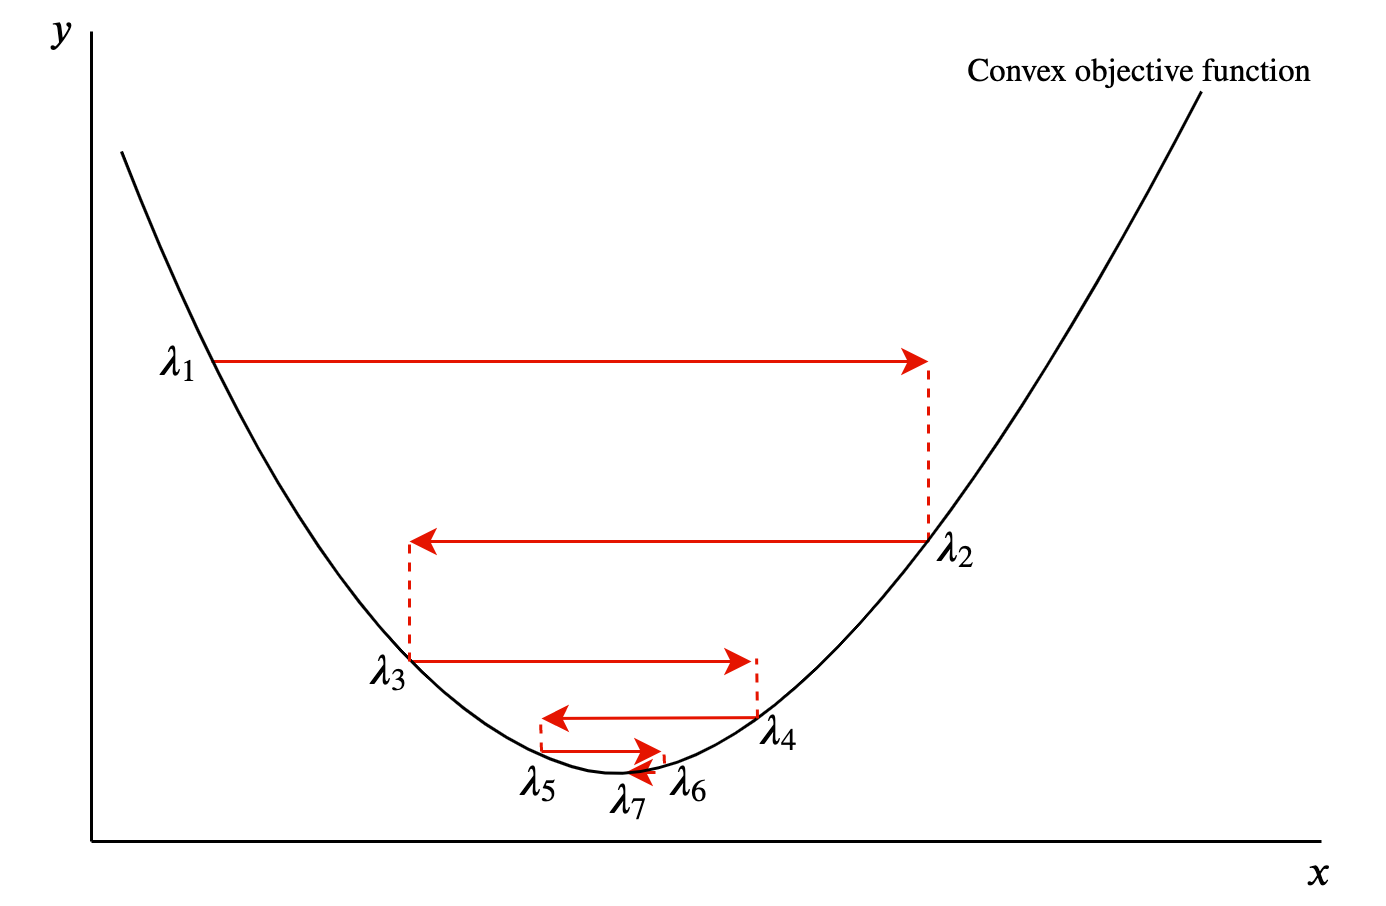
\includegraphics[width=1\linewidth]{images/sgd} \caption{Gradient descent procedure in two dimensions.}\label{fig:gd}
\end{figure}

PD matrices are like the parabola above. Geometrically, they are bowl-shaped and are guaranteed to have a global minimum.\footnote{See these \href{https://www.cis.upenn.edu/~cis515/cis515-12-sl14.pdf}{UPenn lecture notes} for more details.} Consider rolling a ball on the inside surface of this bowl. It would run up and down the edges (losing height each time) before eventually resting on the bottom of the bowl, i.e.~converging on the global minimum. Our algorithm is therefore bound to find the global minimum, and this is obviously a very useful property from an optimisation perspective.

If a matrix is PSD, on the other hand, we are not guaranteed to converge on a global minima. PSD matrices have ``saddle points'' where the slope is zero in all directions, but are neither (local) minima or maxima in all dimensions. Geometrically, for example, PSD matrices can look like hyperbolic parabaloids (shaped like a Pringles crisp). While there is a point on the surface that is flat in all dimensions, it may be a minima in one dimension, but a maxima in another.

PSD matrices prove more difficult to optimise because we are not guaranteed to converge on that point. At a point just away from the saddle point, we may actually want to move in opposite direction to the gradient dependent on the axis. In other words, the valence of the individual elements of the gradient vector point in different directions. Again, imagine dropping a ball onto the surface of a hyperbolic parabaloid. The ball is likely to pass the saddle point then run off one of the sides: gravity is pulling it down in to a minima in one dimension, but away from a maxima in another. PSD matrices therefore prove trickier to optimise, and can even mean we do not converge on a miniimum loss value. Therefore our stable of basic algorithms like GD like gradient descent are less likely to be effective optimisers.

\hypertarget{recap}{%
\subsection{Recap}\label{recap}}

In this final section, we have covered two applications of positive (semi-) definiteness: the proof of OLS as BLUE, and the ease of optimisation when a matrix is PD. There is clearly far more that can be discussed with respect to P(S)D matrices, and this chapter links or cites various resources that can be used to go further.

  \bibliography{book.bib,packages.bib}

\end{document}
